\documentclass[ASNA,twocolumn]{USG}
\usepackage{anyfontsize}
\usepackage{colortbl}
\usepackage{xcolor}
\usepackage{steinmetz}
\usepackage[utf8]{inputenc}
\usepackage[T1]{fontenc}
\usepackage{booktabs}
\usepackage{listings}

\graphicspath{{./images/}}
\specialissue{}
\articletype{REVISIÓN SISTEMÁTICA}
\subarticletype{}
\received{}
\revised{}
\accepted{}
\journal{AIChE Journal}
\volume{0}
\copyyear{2026}
\startpage{1}
\articledoi{}
\begin{document}
	
	\title{Reconocimiento Emocional Facial mediante Aprendizaje Automático para el
		Monitoreo Terapéutico en Niños con Trastorno del Espectro Autista: Una revisión
		sistemática}
	\transtitle{Facial Emotion Recognition through Machine Learning for Therapeutic
		Monitoring in Children with Autism Spectrum Disorder: A systematic review}
	\subtranstitle{}
	
	\author[1,2]{Jorge Eduardo Castañeda Alban}
	\author[1]{Christopher Antonio Pillihuamán Santiago}
	\author[1]{Jhafet Martín Cánepa Maceda}
	\author[3]{Jomark Pablo Noriega Zapata}
	\author[3]{Juan Orlando Salazar Campos}
	\author[4]{Kenny Disney Neira Neira}
	
	\authormark{CASTAÑEDA ALBAN \textsc{et al.}}
	\titlemark{RECONOCIMIENTO EMOCIONAL FACIAL MEDIANTE APRENDIZAJE AUTOMÁTICO}
	
	\address[1]{\orgdiv{Facultad de Ingeniería, }\orgname{Universidad San Ignacio de Loyola, }%
		\orgaddress{\state{Lima, }\country{Perú}}}
	\address[2]{\orgdiv{Programa de Doctorado en Informática, }\orgname{Universidad
			Complutense de Madrid, }%
		\orgaddress{\state{Madrid, }\country{España}}}
	\address[3]{\orgdiv{Facultad de Ingeniería de Sistemas e Informática,
		}\orgname{Universidad Nacional Mayor de San Marcos, }%
		\orgaddress{\state{Lima, }\country{Perú}}}
	\address[4]{\orgdiv{Escuela de Posgrado, }\orgname{Universidad Tecnológica del
			Perú, }%
		\orgaddress{\state{Lima, }\country{Perú}}}
	
	\corres{Jorge Eduardo Castañeda Alban (\email{jorge.castaneda@usil.edu.pe})}
	\editor{}
	\presentaddress{}
	
	\keywords{Trastorno del Espectro Autista | Reconocimiento de Emociones Faciales
		| Aprendizaje Automático | Aprendizaje Profundo | Aplicaciones Móviles de Salud
		| Serious Games | Monitoreo Terapéutico | Redes Neuronales Convolucionales}
	\transkeywords{Autism Spectrum Disorder | Facial Emotion Recognition | Machine
		Learning | Deep Learning | Mobile Health Applications | Serious Games |
		Therapeutic Monitoring | Convolutional Neural Networks}
	
	\abstract[RESUMEN]{Los déficits en el reconocimiento emocional facial constituyen
		una barrera crítica para el monitoreo terapéutico en niños con Trastorno del
		Espectro Autista (TEA). Esta revisión sistemática sintetiza evidencia sobre sistemas
		de reconocimiento de expresividad emocional facial basados en aprendizaje automático
		para el monitoreo terapéutico en niños con TEA. Siguiendo PRISMA 2020, se
		identificaron 1{,}915 registros en Scopus, Web of Science e IEEE Xplore;
		34 estudios publicados entre 2018 y 2025 fueron incluidos. Las arquitecturas CNN
		predominan, con accuracy entre 67.8\% y 88.0\% en datos clínicos genuinos y hasta
		99.0\% en datasets de Kaggle sin validez clínica verificada. Las limitaciones
		críticas incluyen representatividad ecológica limitada (11/34, 32.4\%), desbalance
		de clases (9/34, 26.5\%) y ausencia de datasets validados en Latinoamérica. Esta
		revisión establece fundamentos para desarrollar herramientas digitales accesibles
		y culturalmente adaptadas.%
		\par\smallskip\noindent\textbf{Datasets:} No aplicable (revisión sistemática).
		\textbf{Licencia del Dataset:} No aplicable.}
	
	\transabstract[ABSTRACT]{Deficits in facial emotion recognition constitute a
		critical barrier for therapeutic monitoring in children with Autism Spectrum
		Disorder (ASD). Following PRISMA 2020, 34 studies published between 2018 and 2025
		were selected from 1{,}915 records across Scopus, Web of Science, and IEEE Xplore.
		CNN architectures predominate, reporting accuracy between 67.8\%--88.0\% in
		genuine clinical data versus inflated values up to 99.0\% in Kaggle datasets
		without verified clinical validity. Critical limitations include limited ecological
		representativeness (11/34, 32.4\%), class imbalance (9/34, 26.5\%), and absence
		of validated datasets in Latin America.}
	
	\abbr{TEA, Trastorno del Espectro Autista; CNN, Red Neuronal Convolucional; ML,
		Aprendizaje Automático; LSTM, Long Short-Term Memory; ACC, Exactitud; AUC, Área
		Bajo la Curva; PRISMA, Preferred Reporting Items for Systematic Reviews and
		Meta-Analyses; MMAT, Mixed Methods Appraisal Tool; PICO, Población, Intervención,
		Comparación, Resultado.}
	\contributed{}
	\dedicated{}
	\copyright{© 2026 Los Autores.}
	
	\maketitle
	
	%%=============================================================
	\section{Introducción}\label{sec1}
	%%=============================================================
	
	El Trastorno del Espectro Autista (TEA) es una condición del neurodesarrollo que
	afecta aproximadamente al 1\% de la población mundial, caracterizada por déficits
	persistentes en la comunicación social recíproca y patrones restrictivos de
	comportamiento \cite{Gungor2025}. Entre sus manifestaciones centrales, las
	dificultades en la expresividad emocional facial constituyen uno de los
	predictores más robustos de desafíos en el desarrollo social, afectando
	resultados educativos, relaciones con pares y dinámica familiar \cite{Johnson2025}.
	Investigaciones con tecnologías de seguimiento ocular documentan que niños con
	TEA exhiben patrones diferenciales en el procesamiento de rostros emocionales,
	caracterizados por fijaciones reducidas en la región ocular y procesamiento
	fragmentado de la configuración facial \cite{He2019}, alteraciones que correlacionan
	significativamente con déficits en reconocimiento emocional y teoría de la mente
	\cite{He2019,Reed2021,Lecciso2021}. A pesar de esta evidencia, las intervenciones
	terapéuticas para niños con TEA muestran variabilidad considerable en
	accesibilidad y adaptación cultural, particularmente en entornos con recursos
	limitados, generando una brecha crítica entre la necesidad de monitoreo objetivo
	y las herramientas disponibles para cubrirla \cite{Shaik2025}.
	
	La convergencia de avances en aprendizaje automático, particularmente en Redes
	Neuronales Convolucionales (CNN), y la ubicuidad de dispositivos móviles han
	generado oportunidades para desarrollar herramientas de monitoreo terapéutico
	objetivas y escalables para poblaciones pediátricas. Modelos de transfer learning
	que emplean arquitecturas ResNet-50, EfficientNet y VGGFace han sido aplicados a
	la adaptación a características individuales dentro del espectro autista mediante
	ajuste fino con muestras pequeñas \cite{Ahmad2024}. Sin embargo, la literatura
	revela una paradoja que atraviesa el campo: modelos entrenados en datasets de
	Kaggle sin validez clínica reportan accuracies de hasta 99.0\%, mientras que al
	aplicarse a expresiones faciales atípicas de niños con TEA el rendimiento cae al
	53--74\%, evidenciando una brecha de dominio que limita la transferibilidad de
	estos resultados al contexto terapéutico \cite{Rhatassi2024}. Estudios con datos
	clínicos propios reportan rangos de exactitud entre 67.8\% y 88.0\%, valores más
	modestos pero más representativos de las condiciones reales de uso
	\cite{Johnson2025,Radocaj2025,Washington2022}. Sistemas móviles con OpenCV y
	TensorFlow Lite han sido documentados en entornos naturalistas \cite{Sholikah2024},
	aunque los estudios publicados exhiben heterogeneidad metodológica significativa
	en arquitectura, métricas y poblaciones, lo que limita la comparabilidad directa
	entre enfoques \cite{Radocaj2025}.
	
	Para los fines de esta revisión, el monitoreo terapéutico se define
	operativamente como el seguimiento longitudinal y cuantitativo de la
	expresividad emocional facial de un niño con TEA a lo largo de sesiones de
	intervención, mediante el registro automatizado de patrones emocionales sesión a
	sesión. Este seguimiento permite al terapeuta detectar cambios intraindividuales
	en la frecuencia, intensidad y variabilidad de expresiones emocionales, evaluar
	la respuesta a intervenciones específicas y ajustar las estrategias terapéuticas
	basándose en datos objetivos y reproducibles como complemento a su evaluación
	clínica integral. El monitoreo terapéutico se distingue explícitamente del
	diagnóstico de TEA: no determina ni clasifica el nivel de severidad del trastorno,
	sino que proporciona métricas de progreso terapéutico interpretables por el
	profesional clínico.
	
	Para garantizar consistencia conceptual a lo largo de este documento, se adoptan
	las siguientes definiciones operativas. Reconocimiento emocional facial refiere a
	la capacidad de un sistema computacional de identificar la emoción expresada en
	el rostro de una persona a partir de imagen o video. Expresividad emocional
	refiere a las manifestaciones faciales observables de estados afectivos,
	independientemente de si el sistema las clasifica en categorías discretas.
	Monitoreo terapéutico se definió operativamente en el párrafo anterior.
	Detección de TEA refiere a la clasificación binaria (TEA / no TEA) o por nivel
	de severidad de una condición mediante modelos ML, tarea clínica y
	computacionalmente distinta del monitoreo terapéutico y explícitamente fuera del
	alcance de esta revisión, aunque estudios con este enfoque fueron incluidos como
	contexto comparativo según CI(1).
	
	A pesar de estos avances tecnológicos, la traducción de la investigación a la
	práctica clínica enfrenta barreras críticas en contextos con recursos limitados.
	Una proporción significativa de las aplicaciones para TEA requiere acceso
	constante a Internet, permaneciendo inaccesibles en regiones con infraestructura
	no confiable \cite{Levy2024}. Más aún, el 88\% (30 de 34 estudios) se concentra en
	poblaciones pediátricas menores de 12 años, reflejando un énfasis desproporcionado
	en intervención temprana \cite{Washington2022}. Críticamente, tres estudios fueron
	retractados entre diciembre 2024 y diciembre 2025 debido al uso de datasets de
	Kaggle con imágenes de menores recopiladas de internet sin consentimiento parental
	documentado ni diagnóstico clínico verificado \cite{Gungor2025,Mahmood2025,Kumar2024},
	exponiendo vulnerabilidades éticas fundamentales en la validación de tecnologías
	para TEA. Además, solo 8 de 34 estudios identificados ofrecen algún nivel de
	acceso a datos o código \cite{Sariyanidi2025,Hassan2025}, y ninguno comparte
	simultáneamente dataset completo y código fuente, revelando una crisis de
	reproducibilidad que obstaculiza el progreso científico acumulativo.
	
	La brecha más significativa es la ausencia de herramientas diseñadas para el
	monitoreo terapéutico objetivo: la mayoría de estudios se enfoca en diagnóstico
	binario o clasificación de severidad \cite{Alsubai2025}, enfoque explícitamente
	distinto del monitoreo de progreso terapéutico que constituye el objeto de esta
	revisión, no en métricas de progreso terapéutico sesión a sesión; la evidencia
	específica sobre monitoreo terapéutico de expresividad emocional en TEA es escasa
	dentro del corpus identificado, lo que motiva esta revisión como mapeo del
	panorama existente. Esta brecha es especialmente pronunciada en América Latina,
	donde no existe evidencia de datasets validados culturalmente ni aplicaciones
	adaptadas a contextos con conectividad limitada \cite{Lecciso2021,Rudovic2018}. Esta
	revisión sistemática aborda esta brecha sintetizando arquitecturas ML, métricas
	de rendimiento, características de datasets y limitaciones metodológicas de la
	literatura existente, con el objetivo de establecer fundamentos para herramientas
	de monitoreo terapéutico culturalmente adaptadas al contexto latinoamericano.
	
	%%=============================================================
	\section{Materiales y Métodos}\label{sec2}
	%%=============================================================
	
	\subsection{Preguntas de Investigación y Marco Teórico}\label{sec2a}
	
	A partir de las brechas identificadas en la literatura sobre aplicaciones de
	Aprendizaje Automático (ML) para el reconocimiento de expresividad emocional en
	niños con TEA, se formularon seis Preguntas de Investigación específicas
	(RQ1--RQ6) (Tabla~\ref{tab1}) que articulan motivaciones metodológicas, orientan
	las indagaciones y presentan justificaciones científicas. Estas preguntas
	incorporan métricas de evaluación como precisión, recall, F1-score y Área Bajo la
	Curva (AUC). Para garantizar un análisis riguroso y sistemático, las preguntas
	fueron estructuradas siguiendo el marco Población, Intervención, Comparación,
	Resultado (PICO) adaptado específicamente para revisiones tecnológicas: población
	(niños con TEA), intervención (sistemas ML móviles), comparación (arquitecturas
	alternativas), y resultado (métricas de rendimiento y restricciones de
	implementación).
	
	\begin{table*}[!t]
		\caption{Preguntas de Investigación y Marco Metodológico.\label{tab1}}
		{\setlength{\tabcolsep}{4pt}
			\begin{tabular*}{\textwidth}{@{\extracolsep\fill}lll@{\extracolsep\fill}}
				\toprule
				\textbf{Motivación} & \textbf{Pregunta de Investigación} & \textbf{Justificación} \\
				\midrule
				\parbox[t]{148pt}{Las arquitecturas CNN muestran variabilidad en exactitud (72--96\%) según el diseño, siendo necesario identificar configuraciones óptimas para el monitoreo de expresividad emocional en niños con TEA} &
				\parbox[t]{195pt}{¿Qué arquitecturas subyacentes y modelos de aprendizaje automático han sido empleadas para el reconocimiento de expresividad emocional facial en niños con TEA en el contexto del monitoreo terapéutico?} &
				\parbox[t]{148pt}{Identificar configuraciones técnicas que orienten el diseño de sistemas optimizados para las características específicas del procesamiento emocional en TEA, en el contexto del monitoreo terapéutico} \\[6pt]
				\parbox[t]{148pt}{La heterogeneidad en las métricas reportadas (solo precisión vs.\ F1-score) limita la comparabilidad entre estudios y dificulta establecer estándares para herramientas de apoyo clínico} &
				\parbox[t]{195pt}{¿Qué métricas se emplean para evaluar el rendimiento de los algoritmos, métodos o modelos de reconocimiento emocional?} &
				\parbox[t]{148pt}{Establecer estándares de evaluación que faciliten la comparabilidad entre estudios y la validación clínica en contextos terapéuticos reales} \\[6pt]
				\parbox[t]{148pt}{Los valores absolutos de métricas varían según el rango de edad pediátrico (primera infancia vs.\ infancia media vs.\ adolescencia) y las condiciones de evaluación (laboratorio vs.\ ecológico)} &
				\parbox[t]{195pt}{¿Cuáles son los valores de exactitud, precisión, recall, F1-score y AUC de estos modelos?} &
				\parbox[t]{148pt}{Caracterizar los rangos de rendimiento reportados en la literatura para distintos contextos de evaluación, reconociendo que la heterogeneidad metodológica impide comparaciones directas entre estudios} \\[6pt]
				\parbox[t]{148pt}{Los conjuntos de datos occidentales (FER-2013, CK+) presentan limitaciones de generalización hacia poblaciones latinoamericanas, requiriendo la identificación de alternativas representativas} &
				\parbox[t]{195pt}{¿Qué conjuntos de datos se utilizan para el entrenamiento y validación de modelos, y cuáles son sus limitaciones respecto a la representatividad?} &
				\parbox[t]{148pt}{Evaluar las limitaciones de representatividad y generalización de los datasets disponibles, especialmente respecto a la diversidad cultural y fenotípica relevante para el contexto latinoamericano} \\[6pt]
				\parbox[t]{148pt}{Las variables de entrada (imagen facial únicamente vs.\ multimodal) afectan la robustez de la predicción, requiriendo identificar configuraciones óptimas para implementación móvil en sesiones terapéuticas} &
				\parbox[t]{195pt}{¿Qué variables de entrada o características utilizan los sistemas de monitoreo de expresividad emocional en niños con TEA durante intervenciones terapéuticas?} &
				\parbox[t]{148pt}{Identificar las características de entrada óptimas que equilibren la exactitud del monitoreo con la viabilidad de implementación móvil en entornos con recursos limitados} \\[6pt]
				\parbox[t]{148pt}{Las aplicaciones móviles existentes tienen requisitos técnicos (conectividad, hardware) que limitan la accesibilidad en entornos con recursos restringidos como el contexto latinoamericano} &
				\parbox[t]{195pt}{¿Qué limitaciones técnicas y metodológicas impiden la implementación de sistemas de ML en entornos con recursos limitados?} &
				\parbox[t]{148pt}{Documentar las barreras técnicas, clínicas y de accesibilidad que requieren atención para la traducción efectiva de la investigación en herramientas de apoyo terapéutico funcionales en nuestro contexto} \\
				\bottomrule
		\end{tabular*}}
		\begin{tablenotes}
			\item {\it Nota:} Esta tabla presenta el marco metodológico completo de la revisión
			sistemática, articulando las motivaciones teóricas subyacentes a cada pregunta de
			investigación y sus respectivas justificaciones científicas. Cada pregunta fue
			estructurada siguiendo el marco PICO adaptado para revisiones tecnológicas,
			conectando las brechas identificadas en la literatura con los objetivos específicos
			de síntesis de evidencia orientados al monitoreo de expresividad emocional en
			contextos terapéuticos.
		\end{tablenotes}
	\end{table*}
	
	\subsection{Protocolo y Registro}\label{sec2b}
	
	Esta revisión sistemática fue conducida en conformidad con las directrices PRISMA
	2020 para la presentación integral de revisiones sistemáticas. El protocolo fue
	registrado de manera prospectiva en el Registro Internacional Prospectivo de
	Revisiones Sistemáticas (PROSPERO) bajo el número de registro CRD420251248821.
	Los datos, código y materiales suplementarios están disponibles a través de
	Zenodo (DOI: 10.5281/zenodo.17900467). Se incluyó una lista de verificación
	PRISMA 2020 completa como material suplementario para facilitar la replicación y
	la evaluación metodológica.
	
	\subsection{Fuentes de Información y Estrategia de Búsqueda}\label{sec2c}
	
	Se realizaron búsquedas exhaustivas en tres bases de datos indexadas de
	referencia: IEEE Xplore Digital Library, Scopus y Web of Science Core Collection.
	El período de búsqueda abarcó desde 2019 hasta 2025, incluyendo artículos de
	revista y actas de congresos en las áreas de ciencias de la computación,
	ingeniería biomédica e informática médica. El alcance se restringió a
	publicaciones de acceso abierto con el fin de mejorar la reproducibilidad y
	accesibilidad de los estudios incluidos. Se reconoce que este criterio introduce
	un potencial sesgo de publicación hacia estudios con financiamiento institucional
	para costos de acceso abierto. Las fuentes de literatura gris (preprints, informes
	técnicos y disertaciones) no fueron exploradas sistemáticamente debido a
	restricciones de recursos y consideraciones de control de calidad, lo que podría
	limitar la incorporación de hallazgos emergentes no publicados.
	
	La estrategia de búsqueda fue desarrollada mediante un proceso iterativo que
	incluyó búsquedas piloto. La cadena prioriza los términos centrales del dominio
	(reconocimiento emocional facial, aprendizaje automático, TEA) sobre términos de
	aplicación específica como `serious games' o `therapeutic monitoring', dado que
	la literatura indexada en estas bases de datos raramente emplea dichos términos
	como descriptores primarios en títulos y resúmenes. Una búsqueda piloto con
	términos como `serious game AND autism AND emotion' recuperó menos del 2\% de
	registros adicionales no solapados, confirmando que la cadena principal captura
	adecuadamente el corpus relevante. Se reconoce, no obstante, que esta decisión
	puede haber excluido estudios de intervención terapéutica que emplean terminología
	de gamificación como descriptor principal; esta limitación se documenta
	explícitamente en la Sección~\ref{sec2h}.
	
	La cadena de búsqueda principal empleada en Scopus fue la siguiente:
	
	\begin{boxwithhead}
		{Cadena de búsqueda principal (Scopus)}
		{\noindent\textit{TITLE-ABS-KEY(("autism" OR "ASD" OR "autism spectrum"
				OR "autistic") AND ("emotion" OR "facial expression" OR "affective"
				OR "social communication") AND ("machine learning" OR "deep learning"
				OR "artificial intelligence" OR "computer vision" OR "neural network"
				OR "classification" OR "recognition")) AND PUBYEAR > 2018
				AND PUBYEAR < 2026 AND (LIMIT-TO(DOCTYPE,"ar")
				OR LIMIT-TO(DOCTYPE,"cp")) AND (LIMIT-TO(OA,"all"))
				AND (LIMIT-TO(LANGUAGE,"English"))}}
	\end{boxwithhead}
	
	Esta cadena fue ejecutada con operadores booleanos equivalentes y códigos de
	campo en IEEE Xplore y Web of Science el 15 de febrero de 2026. Las cadenas de
	búsqueda específicas por plataforma se proporcionan en el Material Suplementario
	S1 (disponible en Zenodo, DOI: 10.5281/zenodo.17900467).
	
	\subsection{Criterios de Elegibilidad}\label{sec2d}
	
	Para los fines de esta revisión, la población pediátrica se define como
	individuos de 0 a 18 años, incluyendo primera infancia (0--5 años), infancia
	media (6--11 años) y adolescencia (12--18 años).
	
	\begin{table}[!ht]
		\caption{Aplicación de Criterios de Inclusión y Exclusión.\label{tab2}}
		\begin{tabular*}{\columnwidth}{@{\extracolsep\fill}ll@{\extracolsep\fill}}
			\toprule
			\textbf{Categoría} & \textbf{Rango de Edad} \\
			\midrule
			Primera infancia           & 0--5 años  \\
			Infancia media             & 6--11 años \\
			Adolescencia               & 12--18 años \\
			Población pediátrica total & 0--18 años \\
			\bottomrule
		\end{tabular*}
		\begin{tablenotes}
			\item {\it Nota:} Los rangos de edad fueron definidos siguiendo criterios
			estandarizados de desarrollo pediátrico, reconociendo que cada etapa presenta
			características distintivas en el procesamiento emocional y las manifestaciones
			conductuales del TEA que requieren consideración específica en el diseño de
			intervenciones tecnológicas de monitoreo terapéutico.
		\end{tablenotes}
	\end{table}
	
	Los criterios de inclusión (CI) fueron los siguientes: (1) estudios centrados en
	el reconocimiento de expresividad emocional facial mediante aprendizaje automático
	en niños con TEA, con foco primario en sistemas orientados al monitoreo
	terapéutico de la expresividad emocional; como contexto comparativo secundario se
	incluyeron también estudios orientados a detección o clasificación de TEA,
	exclusivamente para documentar la brecha entre el enfoque diagnóstico predominante
	en la literatura y el enfoque de monitoreo que motiva esta revisión, con la
	restricción explícita de que dichos estudios secundarios quedan excluidos de las
	conclusiones sobre efectividad de herramientas de monitoreo terapéutico y son
	etiquetados como tal en toda la síntesis; (2) empleo de aplicaciones móviles,
	sistemas basados en smartphones o tecnologías adaptables a plataformas móviles;
	(3) reporte de algún resultado cuantitativo de evaluación relevante al diseño del
	estudio: métricas de clasificación supervisada (ACC, F1, AUC) en estudios ML,
	medidas de correlación clínica o tamaño del efecto (ICC, Hedges' g, coeficientes
	de correlación) en estudios clínicos y conductuales, o métricas de usabilidad en
	estudios de diseño de sistemas; (4) publicación en revistas arbitradas o actas de
	congresos indexadas en Scimago Journal Rank (SJR) en cuartiles Q1, Q2, Q3 o Q4;
	(5) disponibilidad como texto completo de acceso abierto; y (6) redactados en
	inglés.
	
	Los criterios de exclusión fueron: (1) artículos de revisión, revisiones
	sistemáticas o metaanálisis; (2) estudios sin validación empírica de ningún tipo,
	es decir, sin reporte de ninguna métrica cuantitativa de evaluación ya sea ML,
	clínica, correlacional o de usabilidad; (3) estudios centrados exclusivamente en
	modalidades no faciales (p.\,ej., únicamente voz o señales fisiológicas sin
	análisis facial); y (4) publicaciones duplicadas del mismo dataset o metodología.
	La aplicación de CI(3) requiere una aclaración metodológica explícita para
	resolver una aparente inconsistencia: los 12 estudios excluidos durante la
	revisión de texto completo bajo este criterio correspondían a trabajos que no
	reportaban ningún tipo de métrica cuantitativa, ni ML ni clínica equivalente. En
	contraste, los 21 estudios incluidos en el corpus final que no reportan métricas
	de clasificación supervisada estándar sí presentan métricas apropiadas a su
	diseño: estudios clínicos reportan tamaños del efecto (Hedges' g = 0.52 en
	\cite{Lecciso2021}), coeficientes de correlación ($r = 0.619$ en \cite{He2019}) o
	coeficientes de confiabilidad inter-evaluador (ICC en \cite{Rudovic2018,Rudovic2019});
	estudios de diseño de sistemas presentan evaluaciones de usabilidad o validación
	de expertos (\cite{Levy2024,Almeida2019}). Esta distinción justifica la inclusión de
	34 estudios pese a que solo 13 reportan métricas de clasificación supervisada
	extraíbles, y es consistente con el criterio CI(3) aplicado de forma diferenciada
	según el tipo de estudio, tal como se documenta en la Tabla~\ref{tab6}.
	
	\subsection{Proceso de Selección y Gestión de Datos}\label{sec2e}
	
	Los registros recuperados fueron importados a un gestor de referencias (Mendeley
	Desktop v1.19.8) y sometidos a eliminación de duplicados mediante algoritmos
	automatizados complementados con verificación manual. El proceso de selección
	siguió un enfoque sistemático en dos fases tal como se documenta en el diagrama
	de flujo PRISMA.
	
	\begin{figure}[htb]
		\centerline{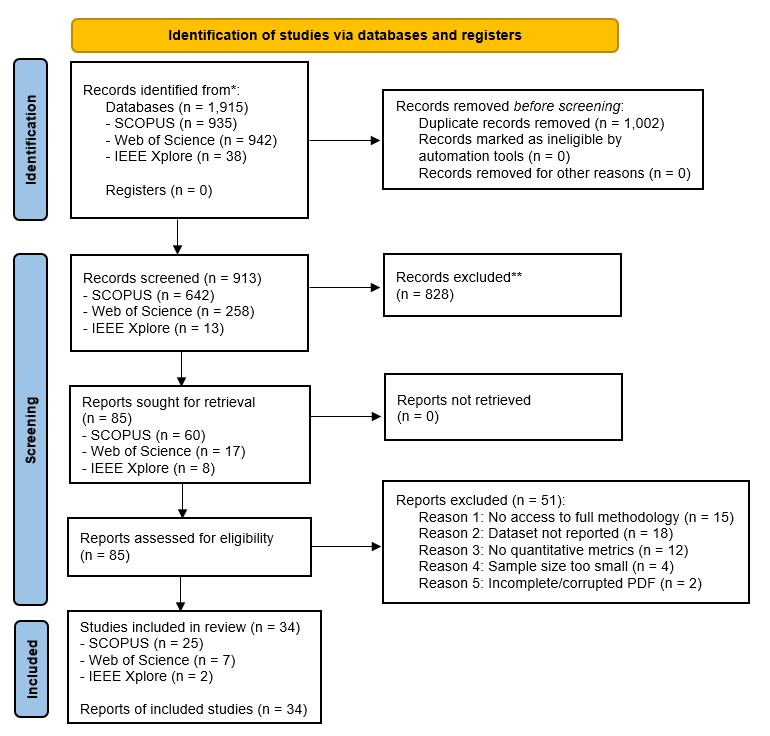
\includegraphics[width=\columnwidth]{fig_1.jpg}}
		\caption{Estrategia de Investigación PRISMA.\\\textit{Nota: La figura ilustra
				el proceso completo de identificación, cribado, elegibilidad e inclusión de
				estudios, desde los 1{,}915 registros iniciales identificados hasta los 34
				estudios finalmente incluidos en la revisión.}\label{fig1}}
	\end{figure}
	
	En la Fase 1 (cribado por título y resumen), dos revisores evaluaron de forma
	independiente todos los registros únicos frente a los criterios de elegibilidad
	mediante un formulario de cribado estandarizado. En la Fase 2 (revisión de texto
	completo), los mismos revisores evaluaron de manera independiente los artículos
	potencialmente elegibles. La confiabilidad entre evaluadores fue monitoreada en
	ambas fases mediante el coeficiente kappa de Cohen ($\kappa = 0.82$ para la Fase
	1; $\kappa = 0.89$ para la Fase 2, indicando acuerdo sustancial a excelente). Las
	discrepancias se resolvieron mediante discusiones estructuradas y los desacuerdos
	no resueltos fueron arbitrados por un tercer revisor senior (J.E.C.A.) con
	experiencia en tecnologías de asistencia e intervenciones para TEA.
	
	Se identificaron 1{,}915 estudios en las tres bases de datos. Tras la eliminación
	de 1{,}002 registros duplicados, quedaron 913 registros para cribado. De estos, 828
	fueron excluidos por título y resumen por no ser relevantes al objetivo de la
	revisión. Los 85 registros restantes fueron evaluados en texto completo, de los
	cuales 51 fueron excluidos por las siguientes razones: 15 sin acceso a metodología
	completa, 18 sin reporte de dataset, 12 sin métricas cuantitativas, 4 con tamaño
	de muestra insuficiente, y 2 con PDF incompleto o corrupto. Finalmente, 34 estudios
	cumplieron todos los criterios de inclusión y fueron retenidos para la síntesis
	cualitativa. La Tabla~\ref{tab3} presenta un resumen cuantitativo de la aplicación
	de los criterios de inclusión y exclusión en todas las fases.
	
	\begin{table*}[!ht]
		\caption{Aplicación de Criterios de Inclusión y Exclusión.\label{tab3}}
		\begin{tabular*}{\textwidth}{@{\extracolsep\fill}llcc@{\extracolsep\fill}}
			\toprule
			\textbf{Criterio} & \textbf{Categoría} & \textbf{N} & \textbf{\%} \\
			\midrule
			\multicolumn{4}{@{}l}{\textit{Criterios de Inclusión Iniciales}} \\
			Actas de congresos   & Identificados & 38      & 1.99\%   \\
			Artículos de revista & Identificados & 1{,}877 & 98.01\%  \\
			\textbf{Subtotal identificados} & & \textbf{1{,}915} & \textbf{100.00\%} \\
			\midrule
			\multicolumn{4}{@{}l}{\textit{Criterios de Exclusión Aplicados}} \\
			Registros duplicados                          & Excluidos & 1{,}002 & 52.32\% \\
			Excluidos por título y resumen (irrelevantes) & Excluidos & 828     & 43.24\% \\
			Sin acceso a metodología completa             & Excluidos & 15      & 0.78\%  \\
			Dataset no reportado                          & Excluidos & 18      & 0.94\%  \\
			Sin métricas cuantitativas                    & Excluidos & 12      & 0.63\%  \\
			Tamaño de muestra insuficiente                & Excluidos & 4       & 0.21\%  \\
			PDF incompleto o corrupto                     & Excluidos & 2       & 0.10\%  \\
			\textbf{Subtotal excluidos} & & \textbf{1{,}881} & \textbf{98.22\%} \\
			\midrule
			\textbf{Total de estudios incluidos en la revisión sistemática} & &
			\textbf{34} & \textbf{1.78\%} \\
			\bottomrule
		\end{tabular*}
		\begin{tablenotes}
			\item {\it Nota:} Los criterios de inclusión priorizan estudios con validación
			empírica cuantitativa publicados en fuentes indexadas de calidad verificable (SJR
			Q1--Q4). Las razones de exclusión en la fase de texto completo fueron aplicadas
			de forma jerarquizada siguiendo el orden establecido en el protocolo: (1) acceso
			a metodología completa, (2) reporte de dataset, (3) métricas cuantitativas,
			(4) tamaño de muestra, (5) integridad del documento. Cada estudio fue asignado a
			la primera categoría de exclusión encontrada durante la revisión; las categorías
			son por tanto mutuamente excluyentes y su suma es trazable al total de 51 estudios
			excluidos en texto completo. Esta jerarquización garantiza consistencia en la
			aplicación del protocolo y permite replicar el proceso de selección a partir de
			la información reportada.
		\end{tablenotes}
	\end{table*}
	
	\subsection{Extracción de Datos y Evaluación de Calidad}\label{sec2f}
	
	Los datos fueron extraídos mediante un formulario estandarizado probado en cinco
	estudios seleccionados aleatoriamente y refinado iterativamente para garantizar
	consistencia e integridad. Para cada estudio incluido se extrajeron
	sistemáticamente: (1) información bibliográfica (autores, año, medio de
	publicación); (2) características de la población del estudio (rango de edad,
	tamaño de muestra, criterios diagnósticos); (3) especificaciones de arquitectura
	y modelo de ML; (4) características de entrada y modalidades de datos; (5)
	conjuntos de datos empleados para entrenamiento y validación; (6) métricas de
	rendimiento reportadas; (7) características de implementación móvil; y (8)
	limitaciones y requisitos técnicos reportados.
	
	Con respecto a los tres estudios retractados identificados
	(\cite{Gungor2025,Mahmood2025,Kumar2024}), se adoptó la siguiente política uniforme:
	estos estudios son documentados en el corpus como evidencia de vulnerabilidades
	éticas críticas en el campo (uso de datasets de menores sin consentimiento
	verificado), pero son excluidos de todos los análisis cuantitativos de rendimiento,
	comparaciones arquitectónicas y síntesis de métricas. Su presencia se limita a
	advertencias éticas en las secciones correspondientes y a la Tabla~16 de
	distribución temporal, donde se identifican explícitamente como categoría separada
	para evidenciar su impacto en el volumen de publicación del período 2024--2025.
	
	Para abordar la evaluación formal de calidad metodológica requerida en revisiones
	sistemáticas rigurosas, se aplicó el Mixed Methods Appraisal Tool (MMAT) versión
	2018 como herramienta de evaluación de calidad estandarizada. El MMAT permite
	evaluar estudios de diseño heterogéneo mediante criterios adaptados al tipo
	metodológico de cada estudio, lo cual resulta apropiado dado que el corpus incluye
	estudios cuantitativos de aprendizaje automático supervisado, estudios clínicos
	observacionales y estudios de diseño de sistemas. Para cada estudio se evaluaron
	cinco criterios de calidad con respuesta S (Sí), N (No) o ND (No Determinable):
	representatividad de la muestra respecto a la población objetivo, adecuación de
	las medidas para responder la pregunta de investigación, ausencia de sesgo de
	selección, control de factores de confusión y completitud de los datos de
	resultado. La evaluación fue realizada de forma independiente por dos revisores y
	las discrepancias fueron resueltas por consenso. Los resultados se presentan en
	la Tabla~\ref{tab4}.
	
	Para estudios de ML supervisado, el criterio Q1 (representatividad de la muestra)
	se evaluó considerando si el dataset empleado corresponde a población pediátrica
	con TEA confirmado clínicamente, o si proviene de fuentes no validadas clínicamente
	como repositorios web. El criterio Q3 (ausencia de sesgo de selección) se evaluó
	considerando los protocolos de partición train/test y la existencia de validación
	cruzada o datasets independientes de prueba. El criterio Q4 (control de factores
	de confusión) se evaluó considerando si los autores controlaron variables como
	iluminación, calidad de imagen, edad y nivel de severidad del TEA en sus análisis.
	Para estudios de diseño de sistemas sin clasificación supervisada, los criterios
	Q3 y Q4 fueron marcados como ND dado que su diseño no contempla las condiciones
	de control propias de estudios cuantitativos experimentales. Es necesario señalar
	una limitación metodológica explícita respecto al uso del MMAT en este corpus: el
	instrumento no fue diseñado para producir scores agregados comparables entre
	diseños de investigación sustancialmente distintos, como estudios de ML supervisado,
	estudios clínicos observacionales y diseños de sistemas. Por esta razón, el score
	/5 reportado en la Tabla~\ref{tab4} no debe interpretarse como una escala ordinal
	de calidad comparable entre tipos de estudio diferentes; su utilidad se restringe
	a identificar dominios específicos de sesgo dentro de cada tipo metodológico y a
	distinguir estudios con fallas éticas o metodológicas fundamentales (score 0--2/5)
	de estudios con mayor rigor en su propio dominio (score 4--5/5). La evaluación
	MMAT se utiliza en esta revisión con ese propósito específico: modular la
	interpretación de resultados y la traslación clínica de cada estudio, tal como se
	desarrolla en la Sección VI.B y la Tabla~17, no para comparar la calidad entre
	estudios de distinta naturaleza metodológica.
	
	\begin{table*}[!ht]
		\caption{Evaluación de Calidad Metodológica mediante MMAT.\label{tab4}}
		\resizebox{\textwidth}{!}{%
			\begin{tabular*}{\textwidth}{@{\extracolsep\fill}clllcccccl@{\extracolsep\fill}}
			\toprule
			\textbf{\#} & \textbf{Referencia} & \textbf{Tipo} & \textbf{Q1} & \textbf{Q2} & \textbf{Q3} & \textbf{Q4} & \textbf{Q5} & \textbf{Score} & \textbf{Estado} \\
			\midrule
			1  & Güngör et al.\ \cite{Gungor2025}            & Cuant.\ no aleatorizado & N  & N  & N  & N  & N  & 0/5 & Retractado \\
			2  & Johnson et al.\ \cite{Johnson2025}           & Cuant.\ no aleatorizado & S  & S  & S  & ND & S  & 4/5 & --- \\
			3  & He et al.\ \cite{He2019}                     & Cuant.\ descriptivo     & S  & S  & S  & S  & S  & 5/5 & --- \\
			4  & Reed et al.\ \cite{Reed2021}                 & Cuant.\ descriptivo     & S  & S  & S  & S  & S  & 5/5 & --- \\
			5  & Lecciso et al.\ \cite{Lecciso2021}           & Mixto                   & S  & S  & S  & ND & S  & 4/5 & --- \\
			6  & Shaik et al.\ \cite{Shaik2025}               & Cuant.\ no aleatorizado & ND & S  & ND & N  & S  & 3/5 & --- \\
			7  & Ahmad et al.\ \cite{Ahmad2024}               & Cuant.\ no aleatorizado & N  & S  & N  & N  & S  & 2/5 & --- \\
			8  & El Rhatassi et al.\ \cite{Rhatassi2024}    & Cuant.\ no aleatorizado & ND & S  & ND & N  & S  & 3/5 & --- \\
			9  & Radočaj \& Martinović \cite{Radocaj2025}     & Cuant.\ no aleatorizado & S  & S  & S  & S  & S  & 5/5 & --- \\
			10 & Washington et al.\ \cite{Washington2022}     & Cuant.\ no aleatorizado & S  & S  & S  & S  & S  & 5/5 & --- \\
			11 & Sholikah et al.\ \cite{Sholikah2024}         & Cuant.\ no aleatorizado & ND & S  & ND & N  & S  & 3/5 & --- \\
			12 & Levy et al.\ \cite{Levy2024}                 & Diseño de sistemas      & ND & S  & ND & ND & ND & 2/5 & --- \\
			13 & Mahmood et al.\ \cite{Mahmood2025}           & Cuant.\ no aleatorizado & N  & N  & N  & N  & N  & 0/5 & Retractado \\
			14 & Kumar et al.\ \cite{Kumar2024}               & Cuant.\ no aleatorizado & N  & N  & N  & N  & N  & 0/5 & Retractado \\
			15 & Sariyanidi et al.\ \cite{Sariyanidi2025}     & Cuant.\ no aleatorizado & S  & S  & S  & S  & S  & 5/5 & --- \\
			16 & Hassan et al.\ \cite{Hassan2025}             & Cuant.\ no aleatorizado & S  & S  & S  & S  & S  & 5/5 & --- \\
			17 & Alsubai \cite{Alsubai2025}                   & Cuant.\ no aleatorizado & N  & S  & N  & N  & S  & 2/5 & --- \\
			18 & Rudovic et al.\ \cite{Rudovic2018}           & Cuant.\ no aleatorizado & S  & S  & S  & S  & S  & 5/5 & --- \\
			19 & Rudovic et al.\ \cite{Rudovic2019}           & Cuant.\ no aleatorizado & S  & S  & S  & S  & S  & 5/5 & --- \\
			20 & Almeida et al.\ \cite{Almeida2019}           & Diseño de sistemas      & ND & S  & ND & ND & ND & 2/5 & --- \\
			21 & Alam et al.\ \cite{Alam2025}                 & Cuant.\ no aleatorizado & ND & S  & N  & N  & S  & 3/5 & --- \\
			22 & Hwang et al.\ \cite{Hwang2024}               & Cuant.\ no aleatorizado & S  & S  & S  & S  & S  & 5/5 & --- \\
			23 & Aljbori et al.\ \cite{Aljbori2025}           & Cuant.\ no aleatorizado & N  & S  & N  & N  & S  & 2/5 & --- \\
			24 & El Rhatassi et al.\ \cite{Rhatassi2025}    & Cuant.\ no aleatorizado & ND & S  & ND & N  & S  & 3/5 & --- \\
			25 & Ramachandran et al.\ \cite{Ramachandran2025} & Cuant.\ no aleatorizado & ND & S  & ND & N  & S  & 3/5 & --- \\
			26 & Hosney et al.\ \cite{Hosney2024}             & Cuant.\ no aleatorizado & N  & S  & N  & N  & S  & 2/5 & --- \\
			27 & Nagae \& Lee \cite{Nagae2022}                & Cuant.\ descriptivo     & S  & S  & S  & ND & S  & 4/5 & --- \\
			28 & Papaioannou et al.\ \cite{Papaioannou2021}   & Cuant.\ descriptivo     & S  & S  & S  & S  & S  & 5/5 & --- \\
			29 & Dapogny et al.\ \cite{Dapogny2019}          & Cuant.\ descriptivo     & S  & S  & S  & S  & S  & 5/5 & --- \\
			30 & Leo et al.\ \cite{Leo2018}                   & Cuant.\ no aleatorizado & S  & S  & S  & S  & S  & 5/5 & --- \\
			31 & Akin-Bulbul et al.\ \cite{AkinBulbul2024}   & Cuant.\ no aleatorizado & S  & S  & S  & ND & S  & 4/5 & --- \\
			32 & Xu \& Ju \cite{Xu2023}                       & Cuant.\ descriptivo     & S  & S  & S  & S  & S  & 5/5 & --- \\
			33 & O'Sullivan et al.\ \cite{OSullivan2023}      & Cuant.\ no aleatorizado & S  & S  & S  & S  & S  & 5/5 & --- \\
			34 & Cicceri et al.\ \cite{Cicceri2026}           & Cuant.\ no aleatorizado & S  & S  & S  & ND & S  & 4/5 & --- \\
			\bottomrule
		\end{tabular*}}
		\begin{tablenotes}
			\item {\it Nota:} S\,=\,Sí; N\,=\,No; ND\,=\,No Determinable. Score indica el
			número de criterios cumplidos sobre 5. Los tres estudios retractados
			(\cite{Gungor2025,Mahmood2025,Kumar2024}) obtienen 0/5 debido a fallos éticos
			fundamentales en la construcción del dataset que comprometen todos los criterios
			de calidad. Los estudios con puntuación 2/5 presentan limitaciones metodológicas
			significativas principalmente en representatividad muestral y control de factores
			de confusión. Los estudios con puntuación 5/5 cumplen todos los criterios
			evaluables según la información reportada en sus publicaciones. La columna Estado
			identifica los estudios formalmente retractados por sus editoriales. Los estudios
			sin observación se indican con ---. Q1: representatividad de la muestra;
			Q2: adecuación de las medidas; Q3: ausencia de sesgo de selección; Q4: control de
			factores de confusión; Q5: completitud de los datos de resultado.
		\end{tablenotes}
	\end{table*}
	
	\subsection{Métodos de Síntesis}\label{sec2g}
	
	La heterogeneidad del corpus hace necesaria una clasificación funcional explícita
	que rija toda la síntesis. Esta clasificación no es un artificio posterior a la
	selección sino el marco estructural que determina qué estudios constituye
	evidencia primaria para cada pregunta de investigación, qué estudios aportan
	contexto comparativo y qué estudios informan el diseño de herramientas
	terapéuticas. Los 34 estudios se clasifican en cuatro categorías: (1)
	reconocimiento emocional facial en TEA mediante ML, categoría de evidencia
	primaria (19 estudios con arquitectura ML identificable orientada a expresividad
	emocional); (2) detección y clasificación de TEA mediante ML, categoría de
	contexto comparativo secundario exclusivamente (\cite{Ahmad2024,Alsubai2025}),
	empleada para evidenciar la brecha entre el enfoque diagnóstico predominante en
	la literatura y el enfoque de monitoreo terapéutico que motiva esta revisión, sin
	que sus resultados constituyan evidencia sobre efectividad de arquitecturas para
	monitoreo; (3) monitoreo terapéutico y sistemas de apoyo clínico, categoría de
	mayor relevancia traslacional directa (\cite{Hassan2025,Rudovic2018,Rudovic2019});
	y (4) estudios clínicos, conductuales y exploratorios sin modelo ML clasificable,
	categoría de referencia ecológica y clínica (7 estudios:
	\cite{He2019,Reed2021,Lecciso2021,Almeida2019,Nagae2022,Papaioannou2021,Xu2023}).
	Las conclusiones orientadas al diseño de herramientas terapéuticas se derivan de
	las categorías 1, 3 y 4; la categoría 2 aporta únicamente contexto comparativo.
	Esta clasificación determina la base de análisis de cada RQ y explica la variación
	en la base N entre preguntas, tal como se documenta en la Tabla~\ref{tab6}.
	
	Dada la considerable heterogeneidad en los diseños de los estudios, arquitecturas
	de ML, conjuntos de datos de evaluación, características de población y métricas
	de resultado, se determinó que un metaanálisis cuantitativo sería inapropiado y
	potencialmente engañoso. En su lugar, se realizó una síntesis descriptiva
	cuantitativa estructurada de las seis preguntas de investigación
	(Tabla~\ref{tab1}). Para cada pregunta, los hallazgos fueron sintetizados mediante
	descripciones narrativas complementadas con tablas resumen y estadísticas
	descriptivas (frecuencias, rangos, medianas según corresponda). Al reportar
	métricas de rendimiento (PI3), se señalaron explícitamente las diferencias en las
	condiciones de evaluación (características del Dataset, tamaños de muestra y
	enfoques de validación) para contextualizar las comparaciones y evitar implicar
	equivalencia directa entre estudios conducidos bajo condiciones heterogéneas.
	Todos los valores de métricas reportados deben interpretarse como resúmenes
	descriptivos del panorama de evidencia actual y no como estimaciones de efecto
	agrupadas.
	
	\subsection{Limitaciones y Sesgos Potenciales}\label{sec2h}
	
	Esta revisión sistemática presenta diversas limitaciones inherentes a su
	metodología. En primer lugar, la restricción a tres bases de datos académicas
	puede haber excluido estudios relevantes indexados en otras fuentes o disponibles
	únicamente en repositorios de literatura gris, limitando potencialmente la
	exhaustividad. En segundo lugar, la restricción a publicaciones de acceso abierto
	constituye una limitación metodológica significativa: aunque mejora la
	reproducibilidad, introduce un sesgo de selección sistemático al excluir
	potencialmente estudios de alto impacto publicados en revistas sin modalidad OA.
	Este sesgo es particularmente grave considerando que la revisión busca abordar el
	contexto latinoamericano, donde los estudios provenientes de regiones con menor
	financiamiento institucional para costos de publicación OA podrían estar
	subrrepresentados. Investigaciones futuras deberían considerar estrategias de
	búsqueda sin esta restricción para obtener un panorama más completo de la
	evidencia disponible. En tercer lugar, la restricción al idioma inglés puede
	resultar en una representación insuficiente de la investigación publicada en otros
	idiomas. En cuarto lugar, la evaluación de la contribución metodológica durante
	la revisión de texto completo, aunque estandarizada mediante pruebas piloto y el
	protocolo de revisión, involucra necesariamente juicio subjetivo informado por la
	experiencia de los revisores en tecnologías de asistencia y aplicaciones clínicas
	para TEA. Finalmente, el sesgo de publicación puede haber influido en los
	hallazgos si estudios con resultados negativos o nulos permanecieron sin publicar,
	inflando potencialmente las métricas de rendimiento observadas en la literatura.
	
	Adicionalmente, la cadena de búsqueda priorizó términos de ML y reconocimiento
	emocional sobre términos de intervención terapéutica y gamificación (p.\,ej.,
	`serious game', `game-based intervention', `therapeutic monitoring', `mHealth').
	Esta decisión requiere una justificación metodológica explícita dado que el
	objetivo declarado de la revisión es precisamente el monitoreo terapéutico: las
	búsquedas piloto con términos como `serious game AND autism AND emotion
	recognition', `therapeutic monitoring AND ASD AND machine learning' y `mHealth
	AND autism AND facial expression' recuperaron en conjunto menos del 2\% de
	registros adicionales no solapados con la cadena principal, lo que indica que la
	literatura de monitoreo terapéutico publicada en las tres bases seleccionadas
	raramente emplea dichos términos como descriptores primarios en títulos y
	resúmenes, recurriendo en cambio a la terminología de ML y reconocimiento
	emocional que caracteriza la cadena empleada. No obstante, se reconoce que esta
	decisión introduce un sesgo potencial de sub-representación de estudios de
	intervención terapéutica que usen gamificación o mHealth como marco principal, lo
	que constituye una limitación directa de este corpus. Para abordarla, se
	recomienda que actualizaciones futuras de esta revisión incluyan una búsqueda
	complementaria en bases de datos especializadas en tecnologías de salud y
	educación (p.\,ej., PsycINFO, CINAHL, Cochrane CENTRAL) con cadenas que combinen
	términos terapéuticos y de gamificación, con el fin de capturar estudios de
	intervención que puedan no estar indexados predominantemente bajo terminología de
	ML en las bases de ciencias de la computación empleadas en esta revisión.
	
	%%=============================================================
	\section{Investigación Actual}\label{sec3}
	%%=============================================================
	
	Los 34 estudios incluidos en esta revisión abordan tareas clínicas y tecnológicas
	heterogéneas; la clasificación funcional adoptada para orientar la síntesis se
	describe en la Sección~\ref{sec2g}. La creciente demanda de herramientas
	tecnológicas para el monitoreo objetivo de la expresividad emocional en niños con
	TEA ha impulsado la generación de volúmenes masivos de datos conductuales,
	fisiológicos y visuales. El análisis de estos datos mediante técnicas de aprendizaje
	automático permite diseñar modelos con potencial clínico significativo para apoyar
	las intervenciones terapéuticas \cite{Johnson2025}. Esta convergencia tecnológica es
	particularmente evidente en el desarrollo acelerado de aplicaciones móviles y
	dispositivos portátiles que permiten procesamiento en tiempo real, operación sin
	conexión en contextos de conectividad limitada, y continuidad terapéutica fuera de
	entornos clínicos controlados \cite{Levy2024}. Las proyecciones del sector sugieren
	un crecimiento exponencial en sistemas de aprendizaje profundo personalizado y
	visión por computador entre 2025 y 2030, impulsado por la maduración de marcos de
	trabajo optimizados para edge computing como TensorFlow Lite y PyTorch Mobile, y la
	proliferación de smartphones con unidades de procesamiento neuronal dedicadas
	\cite{Levy2024}.
	
	La base de evidencia para aplicaciones de ML en el contexto de TEA se concentra
	predominantemente en población infantil. Del total de estudios analizados, el 88\%
	(30 de 34 estudios) se enfocó en niños menores de 12 años, mientras que el 12\%
	restante (4 de 34) incluyó a niños de hasta 18 años. Esta concentración refleja
	tanto el énfasis clínico en la intervención temprana como la disponibilidad de
	protocolos estandarizados de evaluación del desarrollo pediátrico. Los marcos
	metodológicos, los datasets de validación y los benchmarks de rendimiento
	documentados emergen de contextos de investigación enfocados exclusivamente en el
	reconocimiento de expresividad emocional en niños con TEA \cite{Washington2022}.
	
	Diversas investigaciones han abordado los desafíos relevantes de este dominio
	mediante distintos enfoques de ML para la interpretación y toma de decisiones
	\cite{Sariyanidi2025}. Sin embargo, persisten dificultades con los modelos
	implementados \cite{Radocaj2025}, que generalmente siguen paradigmas de caja negra
	con interpretabilidad clínica limitada \cite{Rhatassi2024}. Estos modelos presentan
	problemas particularmente en cuanto a la generalización con muestras pequeñas, el
	desbalance de clases, la multicolinealidad en datos multimodales y la traducción a
	entornos clínicos con recursos limitados \cite{Alam2025}. El desafío radica en
	desarrollar sistemas que equilibren el poder predictivo con la transparencia,
	accesibilidad y adaptación cultural necesarias para contextos como el latinoamericano
	\cite{Shaik2025}.
	
	En la Tabla~\ref{tab5} se resumen los cinco desafíos metodológicos críticos
	identificados en la literatura, junto con los métodos y técnicas de ML propuestos
	para abordarlos, documentando las referencias que reportan explícitamente la
	implementación de estos enfoques. Los enfoques técnicos documentados incluyen:
	Inteligencia Artificial Explicable (XAI) mediante técnicas como LIME, SHAP y
	Grad-CAM para la interpretabilidad de modelos; LSTM para el modelado de secuencias
	temporales; Análisis de Componentes Principales (PCA) y Mínima Redundancia Máxima
	Relevancia (MRMR) para la selección de características; Técnica de Sobremuestreo de
	Minorías Sintéticas (SMOTE), Síntesis Adaptativa (ADASYN), Submuestreo Aleatorio
	(RUS) y Sobremuestreo Aleatorio (ROS) para el balanceo de clases; y validación
	cruzada K-Fold junto con Transfer Learning para la validación y generalización de
	modelos. Esta taxonomía evidencia que, aunque existen métodos para mitigar cada
	limitación individualmente, su aplicación conjunta e integrada en sistemas clínicos
	robustos sigue siendo un área de desarrollo futuro.
	
	\begin{figure*}[htb]
		\centerline{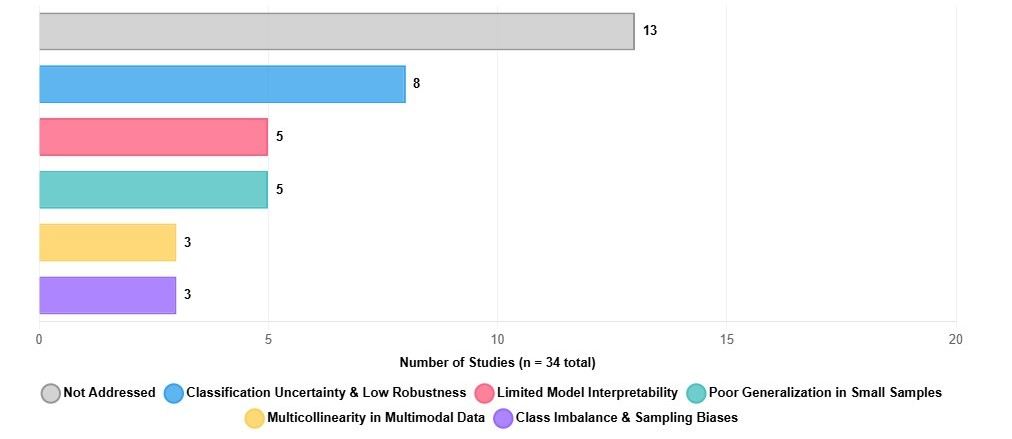
\includegraphics[width=\linewidth]{fig_2.jpg}}
		\caption{Distribución de Estudios que Abordan Desafíos Metodológicos en ML
			para TEA.\\\textit{Nota: La figura presenta un resumen visual de la frecuencia
				con la que los desafíos metodológicos identificados son abordados explícitamente
				en los 34 estudios revisados.}\label{fig2}}
	\end{figure*}
	
	\begin{table*}[!t]
		\centering
		\caption{Desafíos Metodológicos en el Monitoreo de Expresividad Emocional en TEA.\label{tab5}}
		{\setlength{\tabcolsep}{4pt}
			\begin{tabular*}{\textwidth}{@{\extracolsep\fill}clll cc@{\extracolsep\fill}}
				\toprule
				\textbf{\#} & \textbf{Desafío Metodológico} & \textbf{Métodos y Técnicas de ML Propuestos} & \textbf{Estudios (n/34)} & \textbf{Referencias} \\
				\midrule
				1 & \parbox[t]{3.2cm}{Incertidumbre en clasificación y baja robustez predictiva} &
				\parbox[t]{5.5cm}{CNN, Aprendizaje Profundo Personalizado, LSTM, Autoencoders, Visión por Computador} & 7 &
				\cite{Johnson2025,Ahmad2024,Washington2022,Sholikah2024,Sariyanidi2025,Hosney2024,Nagae2022} \\[18pt]
				2 & \parbox[t]{3.2cm}{Interpretabilidad limitada de modelos de caja negra} &
				\parbox[t]{5.5cm}{XAI (LIME, SHAP, Grad-CAM), Importancia de Características, Análisis de Atención} & 3 &
				\cite{Johnson2025,Rhatassi2024,Alam2025} \\[18pt]
				3 & \parbox[t]{3.2cm}{Pobre generalización en muestras pequeñas} &
				\parbox[t]{5.5cm}{K-Fold Cross-Validation, Grid Search, Random Search, Transfer Learning} & 3 &
				\cite{Reed2021,Radocaj2025,Ramachandran2025} \\[18pt]
				4 & \parbox[t]{3.2cm}{Multicolinealidad en datos multimodales correlacionados} &
				\parbox[t]{5.5cm}{PCA, MRMR, Regularización L1/L2, Selección de Características} & 3 &
				\cite{Reed2021,Lecciso2021,Rudovic2019} \\[18pt]
				5 & \parbox[t]{3.2cm}{Desbalance de clases y sesgos de muestreo} &
				\parbox[t]{5.5cm}{SMOTE, RUS, ROS, ADASYN, Ensemble Learning, Aprendizaje Costo-Sensible} & 3 &
				\cite{Radocaj2025,Alam2025,Hosney2024} \\
				\bottomrule
		\end{tabular*}}
		\begin{tablenotes}
			\item {\it Nota:} Los desafíos metodológicos identificados representan limitaciones fundamentales que afectan tanto la validez como la aplicabilidad clínica de los modelos de ML en contextos reales de monitoreo terapéutico. La columna ``Estudios'' indica el número de estudios (sobre 34) que abordan explícitamente cada desafío; los valores no suman 34 porque un mismo estudio puede abordar múltiples desafíos simultáneamente. Cada desafío está vinculado a las técnicas específicas propuestas en la literatura, aunque la implementación conjunta e integrada de estas soluciones en herramientas de apoyo clínico funcionales permanece como área de desarrollo futuro.
		\end{tablenotes}
	\end{table*}
	
	%%=============================================================
	\section{Resultados de la Investigación}\label{sec4}
	%%=============================================================
	
	Para orientar la lectura de los resultados, la Tabla~\ref{tab6} resume la base
	de análisis específica empleada en cada pregunta de investigación, dado que
	distintas RQs operan sobre subconjuntos diferentes del corpus.
	
	\begin{table}[!ht]
		\centering
		\caption{Base de Análisis por Pregunta de Investigación.\label{tab6}}
		{\setlength{\tabcolsep}{3pt}
			\begin{tabular*}{\columnwidth}{@{\extracolsep\fill}llll@{\extracolsep\fill}}
				\toprule
				\textbf{RQ} & \textbf{Estudios analizados} & \textbf{Criterios de exclusión} & \textbf{N} \\
				\midrule
				RQ1 & Arquitecturas ML        & \parbox[t]{2.8cm}{Excluye 8 sin ML, 2 diseño sist., 2 ML no facial, 3 retractados} & 19 \\[18pt]
				RQ2 & Métricas reportadas     & Base total del corpus & 34 \\
				RQ3 & Valores cuantitativos   & \parbox[t]{2.8cm}{Solo estudios con métricas supervisadas extraíbles} & 13 \\[12pt]
				RQ4 & Datasets                & Base total del corpus & 34 \\
				RQ5 & Características entrada & Base total del corpus & 34 \\
				RQ6 & Limitaciones            & Base total del corpus & 34 \\
				\bottomrule
		\end{tabular*}}
		\begin{tablenotes}
			\item {\it Nota:} La variación en la base de análisis entre RQs responde a que cada
			pregunta indaga aspectos distintos del corpus. RQ1 requiere arquitectura ML
			identificable; RQ3 requiere métricas de clasificación supervisada extraíbles. Las
			demás preguntas operan sobre el corpus completo de 34 estudios. Para RQ5, se
			incluyeron los 34 estudios dado que todos reportan características o modalidades
			de datos de entrada, independientemente de si implementan un componente ML
			clasificable. Los 8 estudios clínicos o conductuales aportan información sobre
			variables de entrada conductuales y fisiológicas relevantes para el diseño de
			herramientas de monitoreo terapéutico.
		\end{tablenotes}
	\end{table}
	
	\subsection{Respuesta a RQ1: ¿Qué arquitecturas y modelos de aprendizaje
		automático han sido empleados para el reconocimiento de expresividad emocional
		facial en niños con TEA?}\label{sec4a}
	
	El análisis de los 19 estudios válidos con arquitectura ML identificable reveló
	que los autores emplean predominantemente modelos clasificables en dos categorías
	arquitectónicas según su complejidad: el 73.7\% corresponde a modelos no
	ensamblados (N-Ens) que utilizan arquitecturas individuales, mientras que el
	26.3\% implementa modelos ensamblados (Ens) que combinan múltiples clasificadores
	para mejorar la robustez predictiva mediante votación o apilamiento, tal como se
	detalla en la Tabla~\ref{tab7}. Cabe señalar que los 8 estudios clínicos o
	conductuales sin componente ML, los 2 estudios de diseño de sistemas sin
	clasificación supervisada estándar \cite{Levy2024,Almeida2019}, los 2 estudios con
	modelos ML no orientados al reconocimiento facial o emocional
	\cite{Alsubai2025,OSullivan2023}, y los 3 estudios retractados por irregularidades
	éticas fueron excluidos de este análisis, dado que la RQ1 indaga específicamente
	sobre arquitecturas de aprendizaje automático (ML) aplicadas al reconocimiento
	emocional facial; incluirlos distorsionaría los porcentajes y comprometería la
	validez de las comparaciones arquitectónicas. Dentro de los 19 estudios
	analizados, cuatro corresponden a estudios de detección o screening de TEA
	incluidos como contexto comparativo secundario según CI(1)
	(\cite{Shaik2025,Ahmad2024,Radocaj2025,Alam2025}); sus características
	arquitectónicas se documentan en este análisis para evidenciar la brecha entre el
	enfoque diagnóstico predominante y el enfoque de monitoreo terapéutico, pero las
	conclusiones sobre diseño de herramientas se derivan primariamente de los estudios
	orientados a expresividad emocional y monitoreo, identificados explícitamente en
	la Tabla~17.
	
	\begin{table}[!ht]
		\centering
		\caption{Distribución de Familias de Modelos por Tipo Arquitectónico.\label{tab7}}
		{\setlength{\tabcolsep}{3pt}
			\begin{tabular*}{\columnwidth}{@{\extracolsep\fill}clcccccc@{\extracolsep\fill}}
				\toprule
				\textbf{It.} & \textbf{Familia} & \textbf{Ens} & \textbf{N-E} & \textbf{Tot.} &
				\textbf{E\%} & \textbf{NE\%} & \textbf{T\%} \\
				\midrule
				1 & \parbox[t]{1.8cm}{CNN / Aprendizaje Profundo} & 3 & 8  & 11 & 15.8\% & 42.1\% & 57.9\% \\[12pt]
				2 & ML Tradicional              & 1 & 2  & 3  & 5.3\%  & 10.5\% & 15.8\% \\
				3 & \parbox[t]{1.8cm}{Visión por Comp. / Eye-track.} & 0 & 2 & 2 & 0.0\% & 10.5\% & 10.5\% \\[12pt]
				4 & Multimodal / Wearable       & 1 & 2  & 3  & 5.3\%  & 10.5\% & 15.8\% \\
				& \textbf{Total}              & \textbf{5} & \textbf{14} & \textbf{19} &
				\textbf{26.3\%} & \textbf{73.7\%} & \textbf{100\%} \\
				\bottomrule
		\end{tabular*}}
		\begin{tablenotes}
			\item {\it Nota:} Ens\,=\,Ensamblados; N-E\,=\,No Ensamblados; Tot.\,=\,Total;
			E\%\,=\,Ens\%; NE\%\,=\,N-Ens\%; T\%\,=\,Total\%. La clasificación refleja
			diferencias arquitectónicas fundamentales en complejidad computacional y estrategias
			de predicción. Los modelos no ensamblados fueron los más frecuentemente reportados.
			Se excluyen 8 estudios sin componente ML, 2 estudios de diseño de sistemas
			\cite{Levy2024,Almeida2019}, 2 estudios con ML no orientado al reconocimiento facial
			\cite{Alsubai2025,OSullivan2023} y 3 retractados, quedando 19 estudios como base.
		\end{tablenotes}
	\end{table}
	
	Los modelos se agruparon en cuatro familias según sus principios algorítmicos:
	CNN / Aprendizaje Profundo (57.9\%), que incluye transfer learning con ResNet-50,
	EfficientNet y VGG \cite{Ahmad2024,Radocaj2025}, arquitecturas híbridas CNN-LSTM
	\cite{Aljbori2025,Rhatassi2025} y Vision Transformers \cite{Rhatassi2024,Radocaj2025};
	ML Tradicional (15.8\%), con Random Forest, XGBoost y KNN priorizados por
	interpretabilidad \cite{Hassan2025,AkinBulbul2024}; Visión por Computador /
	Eye-tracking (10.5\%), centrada en landmarks y patrones de fijación
	\cite{Sariyanidi2025,Dapogny2019}; y Multimodal / Wearable (15.8\%), con fusión de
	fuentes heterogéneas para monitoreo continuo \cite{Rudovic2018,Rudovic2019}.
	
	\begin{figure}[htb]
		\centerline{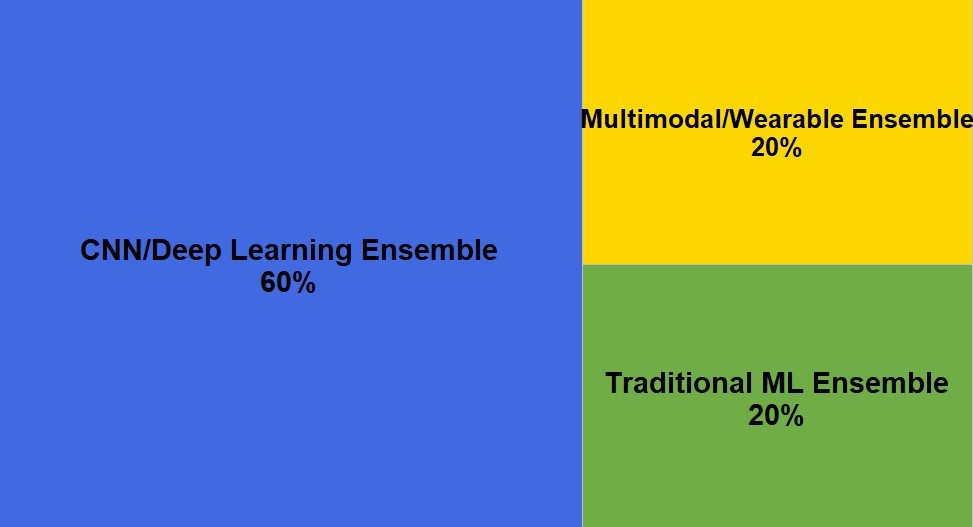
\includegraphics[width=\columnwidth]{fig_3.jpg}}
		\caption{Distribución de Modelos No Ensamblados por Familia Arquitectónica.\\
			\textit{Nota: La figura ilustra la predominancia de arquitecturas CNN /
				Aprendizaje Profundo en implementaciones no ensambladas, reflejando la tendencia
				hacia soluciones basadas en transfer learning para el reconocimiento de
				expresividad emocional en contextos con muestras pequeñas.}\label{fig3}}
	\end{figure}

	
	Entre los modelos no ensamblados, CNN / Aprendizaje Profundo domina con el
	42.1\%, donde el transfer learning desde ImageNet es la estrategia predominante
	para compensar el tamaño reducido de muestras clínicas \cite{Ahmad2024,Washington2022}.
	ML Tradicional y Visión por Computador representan cada uno el 10.5\%,
	persistiendo en escenarios donde la interpretabilidad clínica resulta prioritaria
	\cite{Sariyanidi2025}.
	
	\begin{figure}[htb]
		\centerline{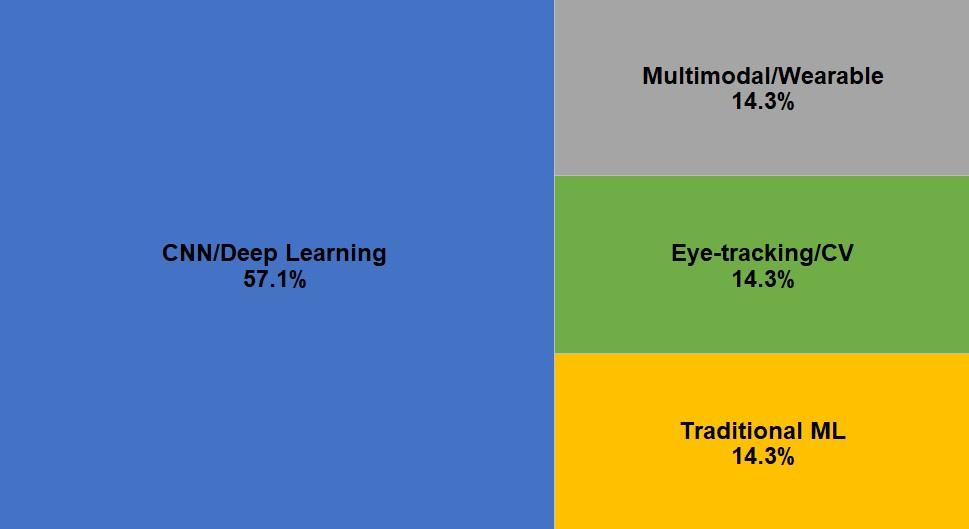
\includegraphics[width=\columnwidth]{fig_4.jpg}}
		\caption{Distribución de Modelos Ensamblados por Familia Arquitectónica.\\
			\textit{Nota: La figura detalla las configuraciones ensambladas identificadas,
				destacando la combinación de clasificadores heterogéneos como estrategia para
				mejorar la robustez predictiva ante la alta variabilidad fenotípica del espectro
				autista.}\label{fig4}}
	\end{figure}
	
	En cuanto a los modelos ensamblados, la familia CNN / Aprendizaje Profundo fue
	implementada en configuraciones ensambladas en el 15.8\% de los estudios, mediante
	técnicas de soft-voting entre múltiples arquitecturas CNN \cite{Shaik2025}, fusión de
	características de tres CNNs con LSTM temporal \cite{Rhatassi2025}, y optimización
	mediante Grey Wolf Optimizer sobre arquitecturas híbridas \cite{Ramachandran2025}.
	El ML Tradicional alcanza el 5.3\% en configuraciones ensambladas a través de
	votación mayoritaria entre Random Forest, XGBoost y Extra Trees \cite{Hassan2025},
	mientras que la familia Multimodal / Wearable representa el 5.3\% mediante la
	fusión de predicciones de múltiples LSTMs especializados por modalidad combinada
	con aprendizaje por refuerzo profundo para la selección activa de datos durante
	sesiones terapéuticas \cite{Rudovic2019}.
	
	Los modelos no ensamblados constituyen el enfoque más frecuentemente reportado en
	la literatura revisada para el reconocimiento de expresividad emocional en TEA. Su
	prevalencia en el corpus puede asociarse con su menor complejidad computacional,
	aunque la frecuencia de uso no equivale a superioridad clínica ni garantiza
	viabilidad de implementación en dispositivos móviles, aspectos que requieren
	validación específica \cite{Sholikah2024}. No obstante, los estudios más recientes
	documentan una tendencia emergente hacia sistemas multimodales que integran
	múltiples fuentes de datos heterogéneas mediante arquitecturas de fusión,
	alcanzando mejoras en la robustez de clasificación de entre 5\% y 15\% respecto a
	enfoques unimodales, especialmente en casos de alta heterogeneidad fenotípica
	característica del espectro autista \cite{Rudovic2019}. Esta tendencia es
	particularmente relevante para el diseño de herramientas de monitoreo terapéutico
	que requieren operar de manera confiable ante la variabilidad expresiva individual
	de cada niño sesión tras sesión.
	
	\subsection{Respuesta a RQ2: ¿Qué métricas se emplean para evaluar el rendimiento
		de los algoritmos, métodos o modelos de reconocimiento emocional?}\label{sec4b}
	
	Se compilaron las métricas reportadas por el modelo principal de cada estudio;
	cuando no se designó uno explícitamente, se reporta el rango observado. La
	distribución se presenta en la Figura~\ref{fig5}.
	
	\begin{figure}[htb]
		\centerline{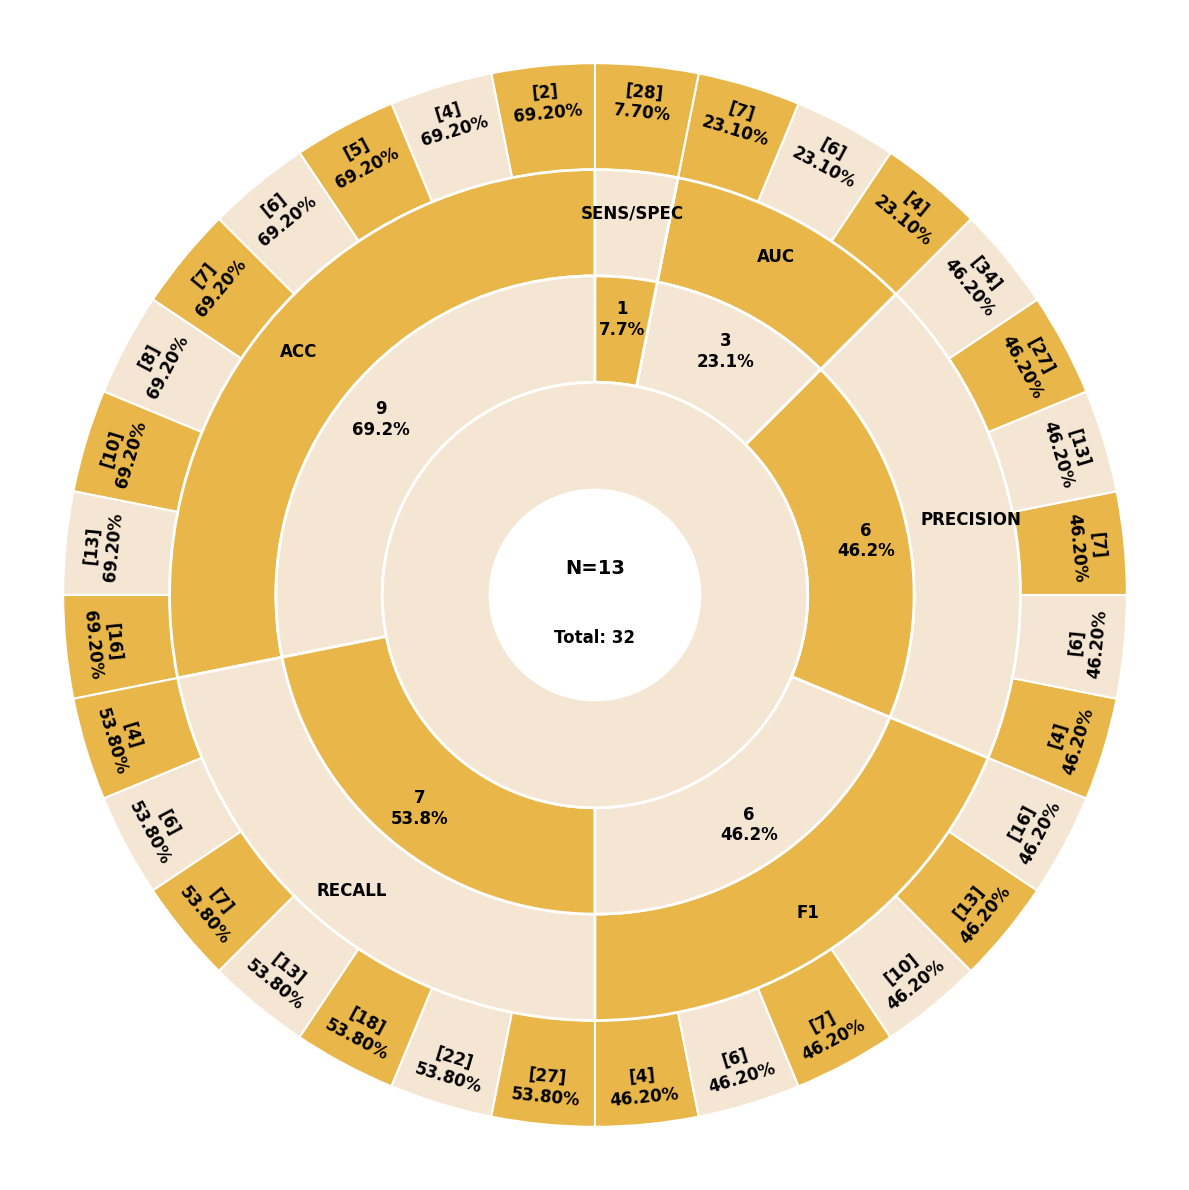
\includegraphics[width=\columnwidth]{fig_5.jpg}}
		\caption{Métricas de Evaluación Utilizadas en los Estudios Analizados.\\
			\textit{Nota: La figura presenta la distribución de frecuencias de las métricas
				reportadas en los estudios con datos cuantitativos de clasificación supervisada,
				evidenciando la predominancia de la exactitud como métrica de referencia y la
				heterogeneidad en los estándares de reporte.}\label{fig5}}
	\end{figure}
	
	Del subconjunto de 13 estudios con métricas de clasificación supervisada
	extraíbles, la Exactitud (ACC) fue la más frecuente (12 estudios), seguida por
	F1-score (9 estudios), Precisión (6 estudios), Recall (4 estudios), AUC (3
	estudios) y la combinación Sensibilidad/Especificidad (1 estudio). La predominancia
	de ACC refleja su interpretabilidad directa, aunque resulta insuficiente ante
	desbalance severo de clases, típico en datos clínicos de TEA. El AUC ofrece
	ventajas metodológicas en ese contexto al evaluar rendimiento independientemente
	del umbral de clasificación, pero su uso sigue siendo minoritario en el corpus. La
	combinación Sensibilidad/Especificidad aparece en estudios orientados a contextos
	clínicos donde el costo diferencial entre falsos positivos y falsos negativos es
	relevante para la toma de decisiones terapéuticas \cite{Leo2018}.
	
	\begin{table*}[!t]
		\centering
		\caption{Métricas Reportadas en 13 Estudios con Datos Cuantitativos de
			Clasificación Supervisada.\label{tab8}}
		{\setlength{\tabcolsep}{4pt}
			\begin{tabular*}{\textwidth}{@{\extracolsep\fill}cllll@{\extracolsep\fill}}
				\toprule
				\textbf{It.} & \textbf{Métrica} & \textbf{N} & \textbf{\%} & \textbf{Autores} \\
				\midrule
				1 & ACC          & 12 & 92\% & \cite{Johnson2025,Shaik2025,Radocaj2025,Washington2022,Sholikah2024,Sariyanidi2025,Hassan2025,Hwang2024,Aljbori2025,Rhatassi2025,Ramachandran2025,Hosney2024} \\
				2 & Precisión    & 6  & 46\% & \cite{Shaik2025,Hwang2024,Aljbori2025,Ramachandran2025,Hosney2024,Cicceri2026} \\
				3 & F1-score     & 9  & 69\% & \cite{Shaik2025,Radocaj2025,Washington2022,Sholikah2024,Hassan2025,Hwang2024,Aljbori2025,Ramachandran2025,Hosney2024} \\
				4 & Recall       & 4  & 31\% & \cite{Shaik2025,Aljbori2025,Ramachandran2025,Hosney2024} \\
				5 & AUC          & 3  & 23\% & \cite{Shaik2025,Aljbori2025,Ramachandran2025} \\
				6 & Sens./Espec. & 1  & 8\%  & \cite{Leo2018} \\
				7 & Otras        & 15 & --   & \cite{He2019,Reed2021,Lecciso2021,Ahmad2024,Rhatassi2024,Levy2024,Alsubai2025,Rudovic2018,Rudovic2019,Almeida2019,Alam2025,Nagae2022,Papaioannou2021,Dapogny2019,AkinBulbul2024} \\
				& \textbf{Total} & \textbf{50} & & \\
				\bottomrule
		\end{tabular*}}
		\begin{tablenotes}
			\item {\it Nota:} La columna N indica el número de estudios que reportaron cada
			métrica específica, mientras que el porcentaje corresponde al total de 13 estudios
			con métricas cuantitativas de clasificación supervisada. Los estudios individuales
			pueden reportar múltiples métricas simultáneamente, por lo que el total no suma 13.
			La categoría ``Otras'' incluye estudios que emplean metodologías cualitativas,
			métricas especializadas no comparables directamente con la clasificación supervisada
			estándar, o estudios clínicos sin modelo ML.
		\end{tablenotes}
	\end{table*}
	
	Estos hallazgos indican que la ACC y las métricas derivadas (Precisión, Recall y
	F1-score) constituyen el estándar de facto para la evaluación de modelos de
	reconocimiento de expresividad emocional en TEA, permitiendo comparaciones entre
	enfoques metodológicos heterogéneos. Sin embargo, persiste una brecha metodológica
	crítica: la ausencia de reporte sistemático de intervalos de confianza, significancia
	estadística de las diferencias entre modelos y análisis de error estratificado por
	subgrupos demográficos. Estas omisiones limitan la interpretabilidad clínica y la
	capacidad de metaanálisis cuantitativo de la literatura existente, dificultando
	además la identificación de rangos de rendimiento referenciales confiables para el
	diseño de herramientas de monitoreo terapéutico en contextos como el latinoamericano
	\cite{Radocaj2025,Hosney2024}.
	
	\subsection{Respuesta a RQ3: ¿Cuáles son los valores de exactitud, precisión,
		recall, F1-score y AUC de estos modelos?}\label{sec4c}
	
	De los 34 estudios, 13 (38.2\%) reportaron métricas cuantitativas de clasificación
	supervisada extraíbles; los 21 restantes emplearon metodologías cualitativas,
	diseños clínicos sin métricas estándar, o fueron excluidos por retracción o
	ausencia de ML. Los valores de la Tabla~\ref{tab9} no constituyen benchmarks
	comparables: provienen de estudios con datasets, tareas clínicas y protocolos
	heterogéneos y deben interpretarse como síntesis descriptiva del panorama actual.
	A efectos interpretativos se distinguen: (a) estudios con datos clínicos o validez
	ecológica verificable (\cite{Johnson2025,Radocaj2025,Washington2022,Sariyanidi2025,Hassan2025,Rudovic2019,Hwang2024}),
	más representativos de condiciones reales de monitoreo; y (b) estudios con datasets
	de Kaggle de validez clínica comprometida
	(\cite{Aljbori2025,Ramachandran2025,Hosney2024}), cuyos valores elevados no son
	transferibles al contexto terapéutico.
	
	\begin{table*}[!t]
		\centering
		\caption{Métricas de Rendimiento Reportadas por Autor.\label{tab9}}
		{\setlength{\tabcolsep}{4pt}
			\begin{tabular*}{\textwidth}{@{\extracolsep\fill}cllllll@{\extracolsep\fill}}
				\toprule
				\textbf{It.} & \textbf{Autor} & \textbf{ACC} & \textbf{Prec.} & \textbf{F1} &
				\textbf{Rec.} & \textbf{AUC} \\
				\midrule
				1  & Johnson et al.\ \cite{Johnson2025}       & 67.8\% & --     & --     & --     & -- \\
				2  & Shaik et al.\ \cite{Shaik2025}           & 84.0\% & 84.8\% & 81.9\% & 86.2\% & 92.3\% \\
				3  & Radočaj \& Martinović \cite{Radocaj2025} & 80.0\% & --     & 78.9\% & --     & -- \\
				4  & Washington et al.\ \cite{Washington2022} & 79.1\% & --     & 78.0\% & --     & -- \\
				5  & Sholikah et al.\ \cite{Sholikah2024}     & 91.0\% & --     & 91.0\% & --     & -- \\
				6  & Sariyanidi et al.\ \cite{Sariyanidi2025} & 83.0\% & --     & --     & --     & -- \\
				7  & Hassan et al.\ \cite{Hassan2025}         & 95.6\% & --     & 92.8\% & --     & -- \\
				8  & Rudovic et al.\ \cite{Rudovic2019}       & --     & --     & --     & --     & -- \\
				9  & Hwang et al.\ \cite{Hwang2024}           & 88.0\% & 91.0\% & 80.0\% & --     & -- \\
				10 & Aljbori et al.\ \cite{Aljbori2025}       & 99.0\% & 98.5\% & 98.6\% & 98.7\% & 99.1\% \\
				11 & El Rhatassi et al.\ \cite{Rhatassi2025}  & 53.0\% & --     & --     & --     & -- \\
				12 & Ramachandran et al.\ \cite{Ramachandran2025} & 96.5\% & -- & 96.4\% & 96.2\% & 96.8\% \\
				13 & Hosney et al.\ \cite{Hosney2024}         & 97.2\% & 94.0\% & 93.0\% & 97.5\% & -- \\
				\bottomrule
		\end{tabular*}}
		\begin{tablenotes}
			\item {\it Nota:} La tabla presenta los valores de las métricas de rendimiento de
			los estudios que reportan datos cuantitativos extraíbles. Se reportan los resultados
			del modelo principal propuesto por los autores. En estudios comparativos sin modelo
			principal designado, se indica el rango. Los valores de algunos estudios pueden
			coincidir con el mejor resultado reportado cuando el modelo principal es también el
			de mejor rendimiento. Los valores vacíos (--) indican que el autor no reportó dicha
			métrica. Los 21 estudios restantes del corpus total de 34 no reportaron métricas
			cuantitativas de clasificación supervisada estándar. Todos los valores se expresan
			en porcentaje. Los valores de \cite{Aljbori2025} y \cite{Hosney2024} deben
			interpretarse con cautela dado que emplean datasets de Kaggle con validez clínica
			comprometida, lo que probablemente infla artificialmente el rendimiento reportado.
			El estudio \cite{Rudovic2019} reporta métricas ACC y F1 en formato gráfico no
			extraíble numéricamente, por lo que todas sus celdas aparecen vacías.
		\end{tablenotes}
	\end{table*}
	
	Los valores de la Tabla~\ref{tab9} no son directamente comparables entre sí. Para
	contextualizar su interpretación, se organizan a continuación según tipo de dataset
	y entorno de evaluación, criterios ya establecidos en la Tabla~17. Los estudios con
	datos clínicos en entorno ecológico o terapéutico real reportan rangos de 67.8\% a
	95.6\% de ACC: Hwang et al.\ \cite{Hwang2024} alcanzaron 88.0\% en aplicación
	móvil con 89 niños; Hassan et al.\ \cite{Hassan2025} reportaron 95.6\% sobre el
	dataset DREAM con más de 3{,}000 sesiones de terapia; Johnson et al.\
	\cite{Johnson2025} reportaron 67.8\% en condiciones naturalistas. Estos valores son
	los más relevantes para el diseño de herramientas de monitoreo por provenir de
	condiciones comparables a las reales. Los estudios con datasets clínicos en
	laboratorio controlado reportan rangos de 79.1\% a 83.0\%: Washington et al.\
	\cite{Washington2022} reportaron 79.1\% sobre el dataset CAFÉ pediátrico; Radočaj
	y Martinović \cite{Radocaj2025} reportaron 80.0\% sobre FERAC; Sariyanidi et al.\
	\cite{Sariyanidi2025} reportaron 83.0\% sobre datos clínicos del Children's
	Hospital of Philadelphia. Los estudios con datasets públicos de benchmark general
	reportan mayor variabilidad: Sholikah et al.\ \cite{Sholikah2024} reportaron 91.0\%
	sobre FER-2013, mientras que El Rhatassi et al.\ \cite{Rhatassi2025} reportaron
	53.0\% de ACC de validación evidenciando overfitting severo, y El Rhatassi et al.\
	\cite{Rhatassi2024} documentaron una caída de 74\% a 65\% al transferir el mismo
	modelo de FER-2013 a datos de población autista, ilustrando la brecha de dominio.
	Finalmente, los estudios con datasets de Kaggle de validez clínica comprometida
	reportan los valores más altos del corpus: 99.0\% \cite{Aljbori2025}, 97.2\%
	\cite{Hosney2024} y 96.5\% \cite{Ramachandran2025}, todos con MMAT 2/5, valores
	no transferibles al contexto terapéutico. Esta organización confirma que a mayor
	validez ecológica del dataset, menor el accuracy reportado pero mayor la relevancia
	traslacional para herramientas de monitoreo en contextos clínicos reales.
	
	\subsection{Respuesta a RQ4: ¿Qué conjuntos de datos se utilizan para el
		entrenamiento y validación de modelos, y cuáles son sus limitaciones respecto a
		la representatividad?}\label{sec4d}
	
	Entre los 34 estudios revisados, los datasets empleados pueden categorizarse según
	su accesibilidad y especificidad de reporte. Al examinar los estudios que
	identificaron explícitamente datasets con nombre, el análisis reveló una
	distribución equilibrada entre fuentes públicas y privadas. Considerando la
	accesibilidad a través de todos los estudios, el 50.0\% involucró datasets
	públicos disponibles a través de repositorios académicos o solicitud directa al
	autor, empleados principalmente para la validación de nuevas arquitecturas ML
	mediante comparación con referencias de rendimiento establecidas. Por contraste,
	el 50.0\% empleó datasets privados o de acceso semirrestringido recopilados ad hoc
	por equipos de investigación específicos, frecuentemente conteniendo datos clínicos
	sensibles o información propietaria que imposibilita su distribución pública, tal
	como se ilustra en la Figura~\ref{fig6}.
	
	\begin{figure}[htb]
		\centerline{
\includegraphics[width=\columnwidth]{fig_6.jpg}}
		\caption{Distribución de Datasets Públicos versus Privados.\\
			\textit{Nota: La figura ilustra la proporción entre datasets públicos y privados
				identificados en los 34 estudios revisados, evidenciando la distribución equilibrada
				entre ambas categorías y la relevancia de los datos clínicos de acceso restringido
				como barrera para la reproducibilidad y el desarrollo de herramientas de monitoreo
				terapéutico en contextos con recursos limitados.}\label{fig6}}
	\end{figure}
	
	\begin{table}[!ht]
		\centering
		\caption{Distribución de Datasets por Accesibilidad.\label{tab10}}
		{\setlength{\tabcolsep}{4pt}
			\begin{tabular*}{\columnwidth}{@{\extracolsep\fill}lcc@{\extracolsep\fill}}
				\toprule
				\textbf{Categoría} & \textbf{Estudios} & \textbf{\%} \\
				\midrule
				\multicolumn{3}{@{}l}{\textit{Datasets Públicos}} \\
				Kaggle ASD / Autistic Children Emotions & 6  & 17.6\% \\
				FER-2013                                & 3  & 8.8\%  \\
				FERAC                                   & 2  & 5.9\%  \\
				CK+ (Extended Cohn-Kanade)              & 1  & 2.9\%  \\
				CAFE                                    & 1  & 2.9\%  \\
				DREAM Dataset                           & 1  & 2.9\%  \\
				ABIDE                                   & 1  & 2.9\%  \\
				Kaggle Screening / Tabulares            & 1  & 2.9\%  \\
				Kaggle FER                              & 1  & 2.9\%  \\
				\textbf{Subtotal Públicos}              & \textbf{17} & \textbf{50.0\%} \\
				\midrule
				\multicolumn{3}{@{}l}{\textit{Datasets Privados / Semirrestringidos}} \\
				Datos clínicos propios (niños ASD)      & 7  & 20.6\% \\
				Datos de terapia con robot              & 3  & 8.8\%  \\
				Datos de eye-tracking clínicos          & 2  & 5.9\%  \\
				Datasets semipúblicos bajo solicitud    & 3  & 8.8\%  \\
				Datos de ensayo clínico corporativo     & 1  & 2.9\%  \\
				Sin dataset ML identificado             & 1  & 2.9\%  \\
				\textbf{Subtotal Privados}              & \textbf{17} & \textbf{50.0\%} \\
				\midrule
				\textbf{Total}                          & \textbf{34} & \textbf{100.0\%} \\
				\bottomrule
		\end{tabular*}}
		\begin{tablenotes}
			\item {\it Nota:} La tabla desglosa la distribución de estudios según la
			accesibilidad de los datasets. Estudios con datasets mixtos fueron asignados a la
			categoría predominante según el componente principal de entrenamiento. Los datasets
			de Kaggle catalogados como públicos incluyen los conjuntos ``Autistic Children
			Emotions'' cuya validez clínica está éticamente comprometida, incluyendo los tres
			estudios retractados \cite{Gungor2025,Mahmood2025,Kumar2024}, lo que debe
			considerarse al interpretar los rendimientos reportados. La categoría ``Datasets
			semipúblicos bajo solicitud'' incluye AffectNet, JEMImE y ALSPAC, que requieren
			solicitud formal al autor o institución.
		\end{tablenotes}
	\end{table}
	
	Dentro del subconjunto de estudios revisados, los datasets públicos y privados se
	distribuyen de manera equilibrada representando cada categoría el 50.0\% del total,
	tal como se detalla en la Tabla~\ref{tab10}. Esta distribución refleja la tensión
	entre los principios de ciencia abierta que favorecen la reproducibilidad mediante
	datasets públicos, y la necesidad práctica de utilizar datos clínicos propietarios
	que capturan la heterogeneidad real de la población pediátrica con TEA en
	condiciones naturalistas. Un hallazgo crítico de esta revisión es que los datasets
	de Kaggle más utilizados, particularmente ``Autistic Children Emotions'' presente
	en al menos seis estudios, presentan vulnerabilidades éticas fundamentales al
	contener imágenes de menores recopiladas de internet sin consentimiento parental
	verificado ni diagnóstico clínico confirmado, lo que originó tres retractaciones
	entre 2024 y 2025 \cite{Gungor2025,Mahmood2025,Kumar2024}.
	
	Entre los datasets públicos disponibles, FER-2013 fue el más frecuentemente
	empleado con una prevalencia del 8.8\% en los estudios revisados, conteniendo
	35{,}888 imágenes de $48\times48$ píxeles etiquetadas en siete categorías
	emocionales. Sin embargo, su uso en el contexto de TEA presenta limitaciones
	críticas de representatividad: fue recopilado exclusivamente de población
	neurotípica occidental, lo que evidencia una brecha de dominio significativa cuando
	se aplica a las expresiones faciales atípicas de niños con TEA. Este fenómeno fue
	documentado directamente por El Rhatassi et al.\ \cite{Rhatassi2024}, donde la
	exactitud cayó de 74\% en FER-2013 a 65\% al aplicar el mismo modelo a datos de
	población autista. El dataset FERAC, con imágenes clínicas de niños con TEA del
	Hospital Ma Shishu en Bangladesh, representa una alternativa metodológicamente más
	sólida al estar recopilado directamente en población objetivo, aunque su tamaño
	reducido limita la generalización \cite{Radocaj2025}. La Figura~\ref{fig7} detalla
	la distribución específica de los datasets más frecuentemente utilizados.
	
	\begin{figure*}[htb]
		\centerline{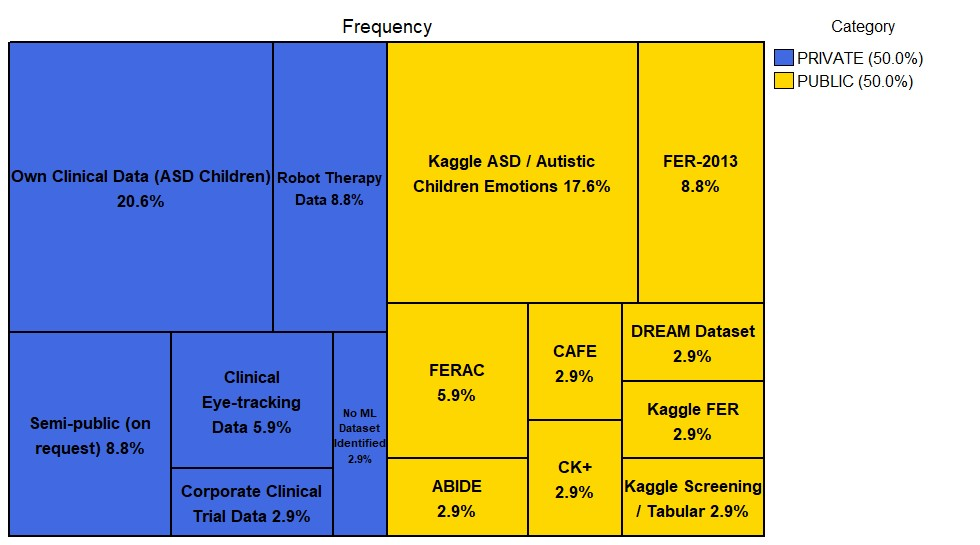
\includegraphics[width=\linewidth]{fig_7.jpg}}
		\caption{Datasets Utilizados en los Estudios Revisados.\\
			\textit{Nota: La figura presenta la distribución de los datasets identificados en
				los 34 estudios, diferenciando entre fuentes públicas y privadas, y señalando
				aquellos con limitaciones éticas o de representatividad que afectan su validez
				para el diseño de herramientas de monitoreo terapéutico.}\label{fig7}}
	\end{figure*}
	
	La industria de aplicaciones de salud móvil y los sistemas de monitoreo terapéutico
	requieren datasets robustos y culturalmente representativos para desarrollar
	herramientas efectivas en contextos como el latinoamericano. Sin embargo, el acceso
	a datasets privados con mayor validez clínica está restringido por consideraciones
	éticas de privacidad bajo normativas como el Reglamento General de Protección de
	Datos (RGPD) y regulaciones equivalentes en América Latina, limitaciones de
	propiedad intelectual de equipos de investigación, y la ausencia de infraestructura
	para compartir datos clínicos sensibles de manera segura
	\cite{Johnson2025,Washington2022}. Esta situación es particularmente crítica para
	el desarrollo de herramientas de monitoreo terapéutico en contextos latinoamericanos,
	donde no existe evidencia de ningún dataset validado que capture la diversidad
	fenotípica y cultural de la población pediátrica con TEA en la región,
	representando una brecha fundamental que impide el desarrollo de sistemas de
	reconocimiento de expresividad emocional culturalmente adaptados para uso terapéutico
	local.
	
	\subsection{Respuesta a RQ5: ¿Qué variables de entrada o características utilizan
		los sistemas de monitoreo de expresividad emocional en niños con TEA durante
		intervenciones terapéuticas?}\label{sec4e}
	
	Los investigadores han propuesto conjuntos heterogéneos de variables de entrada
	empleando diversos métodos para identificar las características con mayor capacidad
	predictiva discriminativa. Las técnicas documentadas incluyen: algoritmos de
	extracción manual de características faciales como Histograma de Gradientes
	Orientados (HOG), Patrones Binarios Locales (LBP) y Transformada de Características
	Invariante a la Escala (SIFT); algoritmos de optimización metaheurística para la
	selección de subconjuntos óptimos de características; métodos estadísticos de
	reducción de dimensionalidad como PCA y Análisis Discriminante Lineal (LDA); y
	arquitecturas de aprendizaje profundo que aprenden representaciones jerárquicas de
	extremo a extremo mediante retropropagación. Los detalles específicos de las
	categorías de características identificadas se presentan en la Tabla~\ref{tab11}.
	
	\begin{table*}[!t]
		\centering
		\caption{Características Específicas Utilizadas.\label{tab11}}
		{\setlength{\tabcolsep}{4pt}
			\begin{tabular*}{\textwidth}{@{\extracolsep\fill}cllcc@{\extracolsep\fill}}
				\toprule
				\textbf{It.} & \textbf{Grupo} & \textbf{Característica} & \textbf{N} & \textbf{\%} \\
				\midrule
				1  & Características Faciales  & Landmarks faciales (68 puntos)           & 4 & 11.8\% \\
				2  & Características Faciales  & Unidades de Acción (AU)                  & 3 & 8.8\%  \\
				3  & Arquitecturas CNN         & CNN personalizada / híbrida              & 3 & 8.8\%  \\
				4  & Características Faciales  & Expresiones emocionales (6--8 clases)    & 3 & 8.8\%  \\
				5  & Arquitecturas CNN         & Transfer Learning (ResNet, EfficientNet, VGG) & 3 & 8.8\% \\
				6  & Características Faciales  & Patrones de gaze / eye-tracking          & 2 & 5.9\%  \\
				7  & Modalidades de Entrada    & Frames de video en tiempo real           & 2 & 5.9\%  \\
				8  & Características Faciales  & Microexpresiones / intensidad expresiva  & 2 & 5.9\%  \\
				9  & Arquitecturas CNN         & Vision Transformer (ViT, Swin)           & 2 & 5.9\%  \\
				10 & Señales Fisiológicas      & GSR / EDA / temperatura periférica       & 1 & 2.9\%  \\
				11 & Características Faciales  & Características geométricas faciales     & 1 & 2.9\%  \\
				12 & Modalidades de Entrada    & Imágenes de smartphone (ecológicas)      & 1 & 2.9\%  \\
				13 & Métodos de Optimización   & HOG + selección de características       & 2 & 5.9\%  \\
				14 & Señales Fisiológicas      & Skeleton 3D + gaze + movimiento de cabeza & 1 & 2.9\% \\
				15 & Modalidades de Entrada    & Video clínico de sesión terapéutica      & 1 & 2.9\%  \\
				16 & Señales Fisiológicas      & Señales EEG                              & 1 & 2.9\%  \\
				17 & Otros                     & Gestos de mano / gesto pointing          & 2 & 5.9\%  \\
				& \textbf{Total}            &                                          & \textbf{34} & \textbf{100.0\%} \\
				\bottomrule
		\end{tabular*}}
		\begin{tablenotes}
			\item {\it Nota:} Las características se organizan por grupos funcionales que
			reflejan la naturaleza algorítmica y la modalidad de datos procesada. La prevalencia
			de características faciales destaca su rol central en el reconocimiento de
			expresividad emocional durante sesiones terapéuticas, mientras que la diversidad
			de enfoques evidencia la heterogeneidad metodológica del campo. Los datos suman 34
			referencias a características principales identificadas, correspondiendo una
			característica predominante por estudio incluido en el corpus.
		\end{tablenotes}
	\end{table*}
	
	Para simplificar el análisis comparativo, las variables propuestas se agruparon en
	seis categorías de alto nivel basadas en su naturaleza algorítmica, tal como se
	sintetiza en la Tabla~\ref{tab12} y se visualiza en la Figura~\ref{fig8}.
	
	\begin{table}[!ht]
		\centering
		\caption{Grupos de Características.\label{tab12}}
		{\setlength{\tabcolsep}{4pt}
			\begin{tabular*}{\columnwidth}{@{\extracolsep\fill}clcc@{\extracolsep\fill}}
				\toprule
				\textbf{It.} & \textbf{Grupo de Características} & \textbf{N} & \textbf{\%} \\
				\midrule
				1 & Características Faciales  & 15 & 44.1\% \\
				2 & Arquitecturas CNN         & 8  & 23.5\% \\
				3 & Modalidades de Entrada    & 4  & 11.8\% \\
				4 & Señales Fisiológicas      & 3  & 8.8\%  \\
				5 & Métodos de Optimización   & 2  & 5.9\%  \\
				6 & Otros                     & 2  & 5.9\%  \\
				& \textbf{Total}            & \textbf{34} & \textbf{100.0\%} \\
				\bottomrule
		\end{tabular*}}
		\begin{tablenotes}
			\item {\it Nota:} Los grupos de características representan categorías de alto
			nivel que consolidan variables específicas basadas en un enfoque algorítmico
			compartido. La marcada preferencia por las características faciales se fundamenta
			en su capacidad para capturar directamente las manifestaciones visibles de la
			expresividad emocional durante sesiones de monitoreo terapéutico, aunque requieren
			complementación con modalidades adicionales para alcanzar un rendimiento clínicamente
			robusto ante la variabilidad fenotípica del espectro autista.
		\end{tablenotes}
	\end{table}
	
	\begin{figure}[htb]
		\centerline{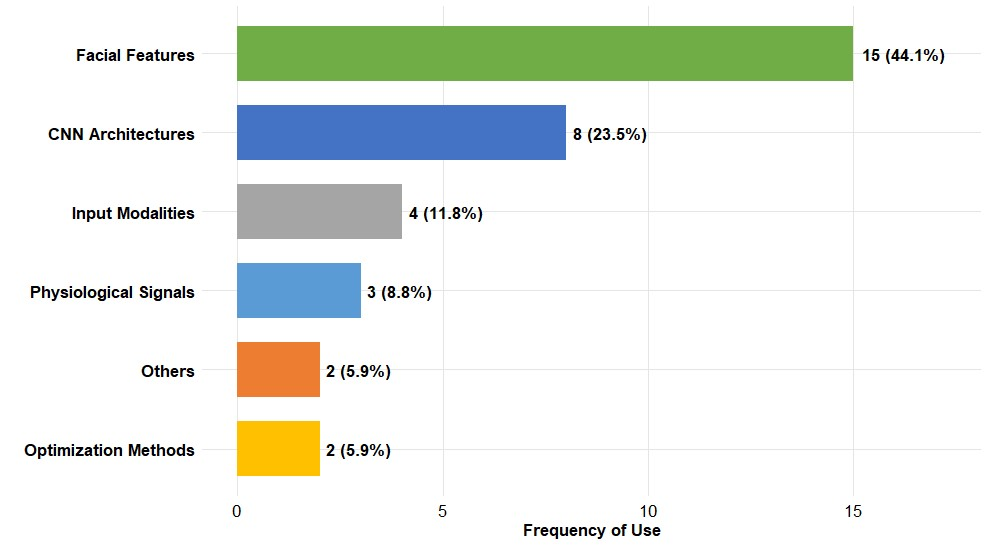
\includegraphics[width=\columnwidth]{fig_8.jpg}}
		\caption{Grupos de Características Utilizadas.\\
			\textit{Nota: La figura presenta la distribución de los grupos de características
				identificados en los 34 estudios incluidos en el corpus, evidenciando la
				predominancia de las características faciales como modalidad principal para el
				reconocimiento de expresividad emocional en niños con TEA.}\label{fig8}}
	\end{figure}
	
	La marcada preferencia por las características faciales para el monitoreo de
	expresividad emocional en población con TEA se fundamenta en que estas modalidades
	pueden capturar directamente las manifestaciones visibles de las expresiones
	emocionales mediante el análisis de configuraciones de Unidades de Acción, detectar
	microexpresiones transitorias de alta frecuencia que revelan estados afectivos
	genuinos antes del enmascaramiento social consciente, e identificar patrones
	atípicos de gaze caracterizados por fijaciones reducidas en la región ocular,
	constituyendo biomarcadores conductuales robustos y observables durante sesiones
	de monitoreo terapéutico \cite{Sariyanidi2025,Leo2018}. Sin embargo, las
	características faciales aisladas resultan insuficientes para alcanzar un
	rendimiento clínicamente robusto ante la heterogeneidad fenotípica del espectro
	autista. Por ello, deben complementarse con arquitecturas CNN adecuadas que capturen
	dependencias espaciales jerárquicas entre regiones faciales, señales multimodales
	que incluyan gestos corporales, patrones de movimiento y contexto social situacional
	de la sesión terapéutica, y técnicas de optimización que permitan una generalización
	efectiva a poblaciones con la amplia variabilidad individual característica del TEA
	\cite{Hassan2025,Rudovic2019}.
	
	\subsection{Respuesta a RQ6: ¿Qué limitaciones técnicas y metodológicas impiden
		la implementación de sistemas de ML en entornos con recursos limitados?}\label{sec4f}
	
	En los artículos revisados sistemáticamente, los autores identificaron explícitamente
	las limitaciones metodológicas o problemas técnicos encontrados durante el diseño,
	implementación y evaluación de sus sistemas experimentales, aunque existen matices
	específicos dependientes del contexto en cada caso. Estas limitaciones heterogéneas
	se consolidaron en seis categorías taxonómicas fundamentales presentadas en la
	Tabla~\ref{tab13}.
	
	\begin{table}[!ht]
		\centering
		\caption{Limitaciones Identificadas en los Estudios Revisados.\label{tab13}}
		{\setlength{\tabcolsep}{3pt}
			\begin{tabular*}{\columnwidth}{@{\extracolsep\fill}clcc@{\extracolsep\fill}}
				\toprule
				\textbf{It.} & \textbf{Limitación Identificada} & \textbf{N} & \textbf{\%} \\
				\midrule
				1 & Representatividad ecológica limitada                  & 11 & 32.4\% \\
				2 & Desbalance de clases y sesgos de muestreo             & 9  & 26.5\% \\
				3 & Inconsistencia en registro y anotación de datos       & 6  & 17.6\% \\
				4 & Interpretabilidad clínica limitada de modelos         & 5  & 14.7\% \\
				5 & Disponibilidad de datos y proc. centralizado          & 2  & 5.9\%  \\
				6 & Adaptabilidad en proc.\ estructurado/no estructurado & 1 & 2.9\% \\[12pt]
				& \textbf{Total}                                        & \textbf{34} & \textbf{100.0\%} \\
				\bottomrule
		\end{tabular*}}
		\begin{tablenotes}
			\item {\it Nota:} Las limitaciones categorizadas representan barreras metodológicas
			y técnicas reportadas explícitamente por los autores en sus publicaciones. La
			representatividad ecológica limitada emerge como la limitación más prevalente,
			reflejando la brecha fundamental entre condiciones experimentales controladas y la
			complejidad dinámica del comportamiento infantil en contextos terapéuticos reales.
			La interpretabilidad clínica limitada constituye una preocupación crítica adicional,
			dado que los terapeutas requieren comprender los mecanismos causales subyacentes a
			las clasificaciones para integrarlas responsablemente en su juicio clínico integral.
		\end{tablenotes}
	\end{table}
	
	La representatividad ecológica limitada, identificada en el 32.4\% de los estudios,
	refiere fundamentalmente a que muchas variables de reconocimiento de expresividad
	emocional evaluadas en protocolos experimentales de laboratorio controlado no
	reflejan plenamente la naturaleza dinámica, dependiente del contexto y socialmente
	situada del comportamiento infantil real durante sesiones terapéuticas. Las
	expresiones emocionales faciales típicamente ocurren en secuencias temporales
	complejas integradas con voz, gestos y contexto social, mientras que los datasets
	de entrenamiento frecuentemente contienen imágenes estáticas aisladas bajo
	condiciones de iluminación artificial uniforme y fondos neutros, generando una
	brecha de validez ecológica que limita la generalización a aplicaciones clínicas
	reales de monitoreo terapéutico \cite{Johnson2025,Radocaj2025}.
	
	El desbalance de clases y sesgos de muestreo, reportado en el 26.5\% de los
	estudios, indica que los datasets clínicos de TEA exhiben típicamente un desbalance
	severo de clases, con proporciones entre 5:1 y 10:1 entre sujetos de desarrollo
	típico y casos de TEA. Esto reduce significativamente el rendimiento de los modelos
	al inducir un sesgo hacia la predicción de la clase mayoritaria, que maximiza la
	exactitud global, pero produce sensibilidad deficiente para la clase minoritaria,
	factor crítico para la utilidad clínica del sistema en contextos de monitoreo
	terapéutico donde la detección de patrones expresivos atípicos resulta prioritaria
	\cite{Alam2025,Hosney2024}.
	
	La inconsistencia en el registro y anotación de datos, observada en el 17.6\% de
	los estudios, refiere a que los registros clínicos existentes han sido anotados
	manualmente con errores humanos sistemáticos, sesgos de anotación entre múltiples
	evaluadores y ruido derivado de protocolos de adquisición no estandarizados. Esto
	requiere técnicas extensivas de limpieza y preprocesamiento de datos con el riesgo
	inherente de perder información crítica durante la normalización o de introducir
	sesgos adicionales mediante decisiones arbitrarias de imputación de valores
	faltantes \cite{Sariyanidi2025,Dapogny2019}.
	
	La interpretabilidad clínica limitada de los modelos, identificada en el 14.7\% de
	los estudios, refiere específicamente a la característica inherente de los modelos
	de aprendizaje profundo como sistemas de caja negra, donde las predicciones emergen
	de interacciones no lineales complejas entre millones de parámetros distribuidos en
	múltiples capas ocultas. Esta opacidad algorítmica obstaculiza profundamente la
	adopción clínica, dado que los terapeutas requieren comprender los mecanismos
	causales subyacentes a las clasificaciones para integrarlas responsablemente en su
	juicio clínico integral y comunicarlas éticamente a las familias de los niños
	atendidos \cite{Rhatassi2024,Radocaj2025}.
	
	Para los modelos de reconocimiento de expresividad emocional aplicados
	específicamente a la población pediátrica con TEA, las dificultades metodológicas
	se concentran en la consistencia y validez ecológica de la información disponible
	para entrenamiento y validación, así como en la ausencia total de datasets
	validados en contextos latinoamericanos. Adicionalmente, la capacidad técnica de
	los modelos para procesar e integrar coherentemente datos multimodales heterogéneos
	representa una limitación fundamental: en esta área clínica especializada, la
	evaluación comprehensiva del progreso terapéutico corresponde necesariamente a la
	integración sinérgica de múltiples señales complementarias incluyendo expresiones
	faciales dinámicas, patrones de movimiento corporal atípicos y contexto situacional
	de la interacción terapéutica \cite{Rudovic2019,Cicceri2026}.
	
	%%=============================================================
	\section{Hallazgos Adicionales}\label{sec5}
	%%=============================================================
	
	A lo largo de esta revisión sistemática se identificaron técnicas de
	preprocesamiento y optimización empleadas de manera recurrente en los experimentos
	analizados. Estos métodos resultan críticos para el rendimiento final de los
	sistemas de reconocimiento de expresividad emocional aplicados a poblaciones
	pediátricas con TEA, aunque con frecuencia son reportados de manera fragmentada o
	con detalle insuficiente en las secciones metodológicas de los estudios.
	
	Las técnicas más prevalentes para la estimación y optimización de hiperparámetros
	corresponden a la Validación Cruzada K-Fold y la Búsqueda en Cuadrícula (Grid
	Search), tal como se documenta en la Tabla~\ref{tab14}. La Validación Cruzada
	K-Fold permite una validación robusta mediante particionamiento iterativo de los
	datos en subconjuntos de entrenamiento y validación, lo cual resulta
	particularmente crítico en los contextos de muestras pequeñas característicos de
	la investigación clínica con TEA, donde los datasets típicamente contienen N menor
	a 100 participantes. La Búsqueda en Cuadrícula explora sistemáticamente el espacio
	de hiperparámetros para identificar configuraciones óptimas, aunque con un costo
	computacional elevado que limita su aplicabilidad en espacios de búsqueda de alta
	dimensionalidad.
	
	\begin{table}[!ht]
		\centering
		\caption{Técnicas para la Determinación de Hiperparámetros.\label{tab14}}
		{\setlength{\tabcolsep}{3pt}
			\begin{tabular*}{\columnwidth}{@{\extracolsep\fill}clccl@{\extracolsep\fill}}
				\toprule
				\textbf{It.} & \textbf{Método} & \textbf{N} & \textbf{\%} & \textbf{Autores} \\
				\midrule
				1 & \parbox[t]{2.2cm}{Validación Cruzada K-Fold} & 8  & 23.5\% & \cite{Shaik2025,Ahmad2024,Radocaj2025,Washington2022,Hassan2025,Alam2025,Rhatassi2025,Ramachandran2025} \\[12pt]
				2 & Grid Search                       & 3  & 8.8\%  & \cite{Radocaj2025,Ramachandran2025,AkinBulbul2024} \\
				3 & Ajuste Manual                     & 4  & 11.8\% & \cite{Johnson2025,Sholikah2024,Aljbori2025,Hosney2024} \\
				4 & Hold-out Validation               & 4  & 11.8\% & \cite{Shaik2025,Sariyanidi2025,Hwang2024,Cicceri2026} \\
				5 & \parbox[t]{2.2cm}{Optim. Metaheurística (GWO)} & 1 & 2.9\% & \cite{Ramachandran2025} \\[6pt]
				6 & No especificado                   & 14 & 41.2\% & -- \\
				& \textbf{Total}                    & \textbf{34} & \textbf{100.0\%} & \\
				\bottomrule
		\end{tabular*}}
		\begin{tablenotes}
			\item {\it Nota:} Los estudios individuales pueden emplear múltiples técnicas
			simultáneamente, resultando en posible superposición entre categorías. Los
			porcentajes reflejan la proporción de estudios que documentaron explícitamente cada
			técnica. La categoría ``No especificado'' incluye estudios que no reportan
			estrategias de validación detalladas o emplean enfoques alternativos no
			clasificables dentro de las técnicas estándar listadas. La Optimización mediante
			Lobo Gris (GWO) corresponde exclusivamente al estudio \cite{Ramachandran2025} que
			implementa esta técnica metaheurística para la selección de hiperparámetros en la
			arquitectura GEfficientNet.
		\end{tablenotes}
	\end{table}
	
	Los algoritmos más empleados para mitigar el desbalance severo característico de
	los datasets clínicos de TEA corresponden a la Aumentación de Datos, seguida de
	SMOTE, Ponderación de Clases y Muestreo Estratificado, tal como se presenta en la
	Tabla~\ref{tab15}. La Aumentación de Datos genera ejemplos sintéticos mediante
	transformaciones geométricas (rotación, traslación, zoom) y fotométricas (ajuste
	de brillo y contraste) de imágenes faciales existentes, aumentando artificialmente
	el tamaño de la clase minoritaria. Por su parte, SMOTE genera instancias sintéticas
	mediante interpolación lineal entre ejemplos vecinos de las clases minoritarias en
	el espacio de características, aunque con el riesgo de generar ejemplos poco
	realistas que no capturan la variabilidad fenotípica real de la expresividad
	emocional en TEA.
	
	\begin{table}[!ht]
		\centering
		\caption{Técnicas de Balanceo de Datasets.\label{tab15}}
		{\setlength{\tabcolsep}{3pt}
			\begin{tabular*}{\columnwidth}{@{\extracolsep\fill}clccl@{\extracolsep\fill}}
				\toprule
				\textbf{It.} & \textbf{Método} & \textbf{N} & \textbf{\%} & \textbf{Autores} \\
				\midrule
				1 & Aumentación de Datos         & 6  & 17.6\% & \cite{Shaik2025,Radocaj2025,Sholikah2024,Aljbori2025,Ramachandran2025,Hosney2024} \\
				2 & SMOTE                        & 2  & 5.9\%  & \cite{Radocaj2025,Alam2025} \\
				3 & Ponderación de Clases        & 3  & 8.8\%  & \cite{Johnson2025,Washington2022,Alam2025} \\
				4 & Muestreo Estratificado       & 3  & 8.8\%  & \cite{Radocaj2025,Rhatassi2025,Ramachandran2025} \\
				5 & \parbox[t]{2.2cm}{Submuestreo Aleatorio (RUS)} & 1 & 2.9\% & \cite{Alam2025} \\[6pt]
				6 & Sin Balanceo Reportado       & 5  & 14.7\% & \cite{Ahmad2024,Levy2024,Alsubai2025,Almeida2019,Nagae2022} \\
				7 & No especificado              & 14 & 41.2\% & -- \\
				& \textbf{Total}               & \textbf{34} & \textbf{100.0\%} & \\
				\bottomrule
		\end{tabular*}}
		\begin{tablenotes}
			\item {\it Nota:} Los estudios individuales pueden emplear múltiples técnicas de
			balanceo simultáneamente, resultando en superposición entre categorías. Los
			porcentajes se calcularon sobre el total de 34 estudios analizados. La categoría
			``No especificado'' incluye estudios que no reportan explícitamente estrategias de
			balanceo o abordan el desbalance mediante métodos alternativos no estandarizados.
		\end{tablenotes}
	\end{table}
	
	El reconocimiento de expresividad emocional en TEA puede conceptualizarse como un
	problema de clasificación supervisada con muestras inherentemente desbalanceadas.
	Dado que la prevalencia del TEA es aproximadamente 1 de cada 36 niños, los estudios
	de monitoreo basados en población inevitablemente generan datasets desbalanceados
	donde la clase mayoritaria (desarrollo típico) supera significativamente a la clase
	minoritaria (TEA) en proporciones que frecuentemente superan 10:1 \cite{Shaik2025}.
	En este contexto, las técnicas de preprocesamiento documentadas en esta revisión
	constituyen una línea base metodológica para nuevas investigaciones orientadas al
	monitoreo terapéutico, considerando que la selección apropiada de técnicas de
	balanceo y optimización de hiperparámetros puede generar mejoras de 10 a 20 puntos
	porcentuales en métricas críticas como Recall y F1-score sin modificar la
	arquitectura subyacente del modelo \cite{Alam2025}.
	
	%%=============================================================
	\section{Discusión}\label{sec6}
	%%=============================================================
	
	\subsection{Arquitecturas de Modelos y Tendencias Temporales}\label{sec6a}
	
	Los modelos de aprendizaje automático más implementados para el reconocimiento de
	expresividad emocional en niños con TEA corresponden a la familia CNN / Aprendizaje
	Profundo, que representa el 57.9\% de las implementaciones con componente ML
	identificable, tal como se documenta en la Tabla~\ref{tab16} y se visualiza en la
	Figura~\ref{fig9}. Esta distribución refleja la convergencia entre accesibilidad
	práctica y madurez metodológica: los modelos CNN no ensamblados fueron los más
	frecuentemente reportados en la literatura revisada. Esta prevalencia puede estar
	relacionada con su menor costo computacional, aunque la frecuencia de uso no
	equivale a superioridad clínica ni garantiza viabilidad de implementación en
	dispositivos móviles \cite{Sholikah2024}. Los modelos que alcanzan los mayores
	resultados cuantitativos corresponden a configuraciones ensambladas que combinan
	CNN con LSTM temporal y fusión multimodal, alcanzando exactitudes superiores al
	95\% en datasets controlados, aunque estos valores deben interpretarse con
	considerable cautela dado que provienen predominantemente de datasets de Kaggle con
	validez clínica comprometida \cite{Aljbori2025,Ramachandran2025}. Los estudios con
	mayor relevancia traslacional para el monitoreo terapéutico, como Hassan et al.\
	\cite{Hassan2025} y Hwang et al.\ \cite{Hwang2024}, reportan rangos más modestos
	(88--95.6\%) pero sobre datos clínicos genuinos en contextos de terapia real.
	
	\begin{table*}[!t]
		\centering
		\caption{Tendencias de Familias de Modelos por Año.\label{tab16}}
		{\setlength{\tabcolsep}{4pt}
			\begin{tabular*}{\textwidth}{@{\extracolsep\fill}clccccccccc@{\extracolsep\fill}}
				\toprule
				\textbf{It.} & \textbf{Familia} & \textbf{2018} & \textbf{2019} & \textbf{2021} &
				\textbf{2022} & \textbf{2023} & \textbf{2024} & \textbf{2025} & \textbf{2026} &
				\textbf{Total} \\
				\midrule
				1 & CNN / Deep Learning                    & 0 & 0 & 0 & 1 & 0 & 5  & 7  & 0 & 13 \\
				2 & ML Tradicional                         & 0 & 1 & 0 & 0 & 0 & 2  & 0  & 0 & 3  \\
				3 & Visión por Computador / Eye-tracking   & 1 & 0 & 0 & 0 & 0 & 0  & 1  & 0 & 2  \\
				4 & Multimodal / Wearable                  & 1 & 1 & 0 & 1 & 0 & 0  & 1  & 1 & 5  \\
				5 & Sin modelo ML (clínicos/conceptuales)  & 0 & 2 & 3 & 0 & 2 & 0  & 1  & 0 & 8  \\
				6 & Retractados                            & 0 & 0 & 0 & 0 & 0 & 1  & 2  & 0 & 3  \\
				& \textbf{Total}                         & \textbf{2} & \textbf{4} & \textbf{3} &
				\textbf{2} & \textbf{2} & \textbf{8} & \textbf{12} & \textbf{1} & \textbf{34} \\
				\bottomrule
		\end{tabular*}}
		\begin{tablenotes}
			\item {\it Nota:} La distribución temporal muestra una concentración de
			productividad entre 2024 y 2025, coincidiendo con la maduración de marcos de
			trabajo de aprendizaje profundo optimizados para dispositivos móviles y la
			proliferación de smartphones con unidades de procesamiento neuronal dedicadas.
			Los estudios sin modelo ML incluyen estudios clínicos, conductuales y de diseño
			de sistemas sin componente de clasificación supervisada.
		\end{tablenotes}
	\end{table*}
	
	\begin{figure*}[htb]
		\centerline{
\includegraphics[width=\linewidth]{fig_9.jpg}}
		\caption{Evolución Temporal de las Implementaciones de Familias de Modelos ML
			(2018--2026).\\\textit{Nota: La figura visualiza la distribución anual de los 34
				estudios incluidos por familia de modelo, evidenciando la aceleración reciente en
				implementaciones CNN/Deep Learning y la concentración de productividad entre 2024
				y 2025.}\label{fig9}}
	\end{figure*}
	
	El análisis temporal revela una concentración de productividad entre 2024 y 2025,
	coincidiendo con la maduración de frameworks de aprendizaje profundo optimizados
	para dispositivos móviles como TensorFlow Lite y PyTorch Mobile, y la proliferación
	de smartphones con unidades de procesamiento neuronal dedicadas. Esta concentración
	temporal refleja la maduración reciente de las tecnologías ML para aplicaciones
	clínicas y el reconocimiento creciente de las plataformas móviles como vehículos
	viables para intervenciones terapéuticas continuas fuera de entornos clínicos
	controlados \cite{Levy2024}.
	
	Un patrón descriptivo que emerge del análisis del corpus es que los estudios que
	emplean arquitecturas híbridas CNN-LSTM en configuraciones multimodales reportan
	valores de F1-score entre 8\% y 15\% superiores a los reportados por estudios que
	emplean CNNs individuales \cite{Rhatassi2025,Rudovic2019}. Sin embargo, dado que
	estos estudios difieren en dataset, población, entorno de evaluación y protocolo
	de validación, esta diferencia numérica no puede interpretarse como evidencia de
	superioridad arquitectónica; refleja únicamente que distintas combinaciones de
	arquitectura, dataset y contexto producen distintos valores de métricas bajo
	condiciones no controladas de forma equivalente. Lo que sí puede afirmarse
	descriptivamente es que los estudios con mayor validez ecológica documentada, como
	Hwang et al.\ \cite{Hwang2024}, Hassan et al.\ \cite{Hassan2025} y Rudovic et al.\
	\cite{Rudovic2019}, emplean arquitecturas que integran modelado temporal y fusión
	multimodal en contextos terapéuticos reales, lo cual constituye una referencia
	metodológica para el diseño de nuevas herramientas, no una demostración de
	efectividad comparativa.
	
	\subsection{Métricas de Evaluación y Datasets}\label{sec6b}
	
	La tesis metodológica central de esta revisión, sostenida por el análisis conjunto
	de métricas de rendimiento, evaluación MMAT y tipo de dataset, es la siguiente:
	existe una correlación inversa sistemática entre el accuracy reportado y la validez
	clínica y ecológica del estudio, de modo que a mayor validez del dataset y del
	entorno de evaluación, menor el rendimiento aparente pero mayor la utilidad
	traslacional al contexto terapéutico real. Esta tesis tiene implicancias directas
	para el diseño de herramientas de monitoreo terapéutico: un sistema que optimiza
	accuracy sobre datasets de Kaggle no es necesariamente un mejor candidato para
	implementación clínica que uno que reporta 15 puntos menos sobre datos pediátricos
	genuinos en condiciones ecológicas.
	
	La evidencia que sostiene esta tesis es la siguiente. De los tres estudios
	retractados entre 2024 y 2025, Mahmood et al.\ \cite{Mahmood2025} reportaron
	91.33\% de ACC con datos de Kaggle sin validez clínica; Güngör et al.\
	\cite{Gungor2025} reportaron 75.8\% con el mismo dataset combinado con FERAC; y
	Kumar et al.\ \cite{Kumar2024} reportaron 79.56\% de mAP con imágenes de internet
	sin diagnóstico verificado; los tres fueron retractados por uso de imágenes de
	menores sin consentimiento documentado. Aljbori et al.\ \cite{Aljbori2025} y
	Hosney et al.\ \cite{Hosney2024}, también con datos de Kaggle, reportan valores de
	99.0\% y 97.2\% respectivamente, ambos con MMAT 2/5. En el extremo opuesto, los
	estudios con mayor validez clínica y ecológica reportan rendimientos entre 67.8\%
	y 88.0\%: Hwang et al.\ \cite{Hwang2024} alcanzaron 88.0\% con 89 niños en
	condiciones ecológicas reales (MMAT 5/5); Washington et al.\ \cite{Washington2022}
	reportaron 79.1\% de balanced accuracy con el dataset CAFÉ pediátrico (MMAT 5/5);
	Johnson et al.\ \cite{Johnson2025} reportaron 67.8\% en condiciones naturalistas
	con niños con TEA (MMAT 4/5). El patrón es consistente: MMAT 0--2/5 corresponde a
	accuracy 91--99\%, MMAT 4--5/5 corresponde a accuracy 67--88\%.
	
	Ejemplificando con mayor detalle: Aljbori et al.\ \cite{Aljbori2025} reportan
	99.01\% de ACC sobre un dataset de Kaggle de 6 categorías emocionales cuya
	procedencia ética no está verificada; Hosney et al.\ \cite{Hosney2024} reportan
	97.2\% sobre un dataset creado por una co-autora del mismo estudio, constituyendo
	un conflicto de interés documentado; El Rhatassi et al.\ \cite{Rhatassi2025}
	reportan 94.5\% de ACC en entrenamiento que colapsa a 53.03\% en validación,
	exponiendo overfitting severo. Esto no es coincidencia metodológica sino reflejo
	de que los datos clínicamente válidos capturan la variabilidad real de la
	expresividad emocional en TEA, que es inherentemente más difícil de clasificar que
	poses controladas de Kaggle. El desarrollo de herramientas de monitoreo terapéutico
	debe por tanto priorizar la validez ecológica del dataset sobre la optimización de
	métricas en laboratorio, aceptando rangos de rendimiento más modestos como
	consecuencia natural de trabajar con datos clínicamente representativos.
	
	Las métricas de evaluación más prevalentes fueron la Exactitud (ACC), reportada en
	12 de 13 estudios (92\%); la F1-score, en 9 de 13 estudios (69\%); la Precisión,
	en 6 de 13 estudios (46\%); el Recall, en 4 de 13 estudios (31\%); y el AUC, en 3
	de 13 estudios (23\%). Esta distribución puede explicarse por la mayor familiaridad
	de los investigadores con las métricas estándar de clasificación y la
	interpretabilidad directa de la ACC para audiencias clínicas. Sin embargo, el AUC
	ofrece ventajas metodológicas fundamentales en el contexto de desbalance severo de
	clases al evaluar el rendimiento independientemente del umbral de clasificación
	seleccionado \cite{Radocaj2025,Hosney2024}.
	
	Los datasets públicos más utilizados corresponden a FER-2013 (8.8\%) y FERAC
	(5.9\%), empleados principalmente para la validación de nuevas arquitecturas
	mediante comparación con referencias de rendimiento establecidas. Los datasets
	privados representan el 50.0\% de las implementaciones, generando conocimiento a
	través de aplicaciones en escenarios clínicos específicos que reflejan
	heterogeneidad real de la población pediátrica con TEA. Una limitación crítica es
	la ausencia total de datasets públicos que incluyan población pediátrica
	latinoamericana con TEA, comprometiendo la generalización de modelos entrenados
	predominantemente en datasets occidentales hacia contextos culturales donde las
	expresiones emocionales infantiles pueden manifestarse de manera diferente. Además,
	el 88\% de los estudios revisados (30 de 34) se concentró en niños menores de 12
	años, indicando la necesidad de ampliar la investigación hacia grupos de edad
	pediátrica mayor.
	
	Las limitaciones principales identificadas en los datasets corresponden a
	representatividad ecológica limitada (32.4\%), reflejando una brecha entre las
	condiciones de laboratorio controlado y la variabilidad del contexto real de
	sesiones terapéuticas; desbalance severo de clases (26.5\%), que introduce sesgos
	predictivos hacia las clases mayoritarias; e inconsistencia en el registro de datos
	(17.6\%) debida a errores de anotación, protocolos no estandarizados y variabilidad
	entre evaluadores.
	
	La evaluación de calidad metodológica mediante MMAT revela una distribución
	polarizada en el corpus analizado. Los estudios con mayor rigor metodológico
	(puntuación 5/5) corresponden predominantemente a investigaciones clínicas con
	datos propios, muestras clínicamente validadas y protocolos de evaluación
	controlados (\cite{He2019,Reed2021,Hwang2024,Radocaj2025,Washington2022,Sariyanidi2025,Hassan2025,Rudovic2018,Papaioannou2021,Rudovic2019,Dapogny2019,Leo2018,Xu2023,OSullivan2023}).
	En contraste, los estudios con puntuaciones bajas (0--2/5) corresponden a los tres
	retractados y a estudios que emplean datasets de Kaggle sin representatividad
	clínica verificada, sin control de factores de confusión y con sesgos de selección
	evidentes. Esta distribución confirma la paradoja accuracy-calidad identificada en
	RQ3: los estudios con mayor rendimiento reportado tienden a tener menor rigor
	metodológico, mientras que los estudios con mayor calidad metodológica reportan
	rendimientos más modestos, pero clínicamente más transferibles. Esta heterogeneidad
	de calidad debe considerarse al interpretar cualquier síntesis de la evidencia y
	refuerza la necesidad de estándares de reporte más rigurosos en la literatura sobre
	ML aplicado a TEA.
	
	Esta distribución de calidad tiene implicancias directas para la interpretación de
	los hallazgos de esta revisión. Los resultados de estudios con puntuación 5/5, como
	Hwang et al.\ \cite{Hwang2024}, Washington et al.\ \cite{Washington2022}, Hassan
	et al.\ \cite{Hassan2025} y Rudovic et al.\ \cite{Rudovic2018,Rudovic2019}, ofrecen
	evidencia más sólida para orientar el diseño de herramientas de monitoreo
	terapéutico, dado que sus metodologías son clínicamente verificables y sus datasets
	tienen validez ecológica documentada. En contraste, los valores de rendimiento
	reportados por estudios con puntuación 2/5 o inferior, como Aljbori et al.\
	\cite{Aljbori2025}, Hosney et al.\ \cite{Hosney2024} y los tres retractados, deben
	considerarse no transferibles al contexto clínico real. Por tanto, en esta revisión
	se priorizan los hallazgos de estudios de mayor calidad metodológica al formular
	implicancias para el diseño de herramientas terapéuticas.
	
	\subsection{Características de Entrada y Limitaciones}\label{sec6c}
	
	Las variables más prevalentes para el reconocimiento de expresividad emocional
	correspondieron a las Características Faciales (44.1\%), las Arquitecturas CNN
	(23.5\%) y las Modalidades de Entrada de video (11.8\%), tal como se muestra en
	las Tablas~\ref{tab11} y \ref{tab12}. Esta distribución indica que las
	características faciales proporcionan información discriminativa directa sobre las
	expresiones emocionales, mientras que las arquitecturas CNN permiten la extracción
	automática de representaciones jerárquicas sin ingeniería manual de características.
	Sin embargo, las señales fisiológicas complementarias (8.8\%) y las características
	contextuales permanecen subutilizadas a pesar de su potencial para capturar
	manifestaciones autonómicas de estados emocionales no visibles en expresiones
	faciales, aspecto particularmente relevante en TEA donde puede existir disociación
	entre la experiencia emocional interna y la expresión facial externa
	\cite{Rudovic2018,Rudovic2019}.
	
	Las limitaciones metodológicas fundamentales identificadas, incluyendo
	representatividad ecológica limitada (11 de 34, 32.4\%), desbalance de clases
	(9 de 34, 26.5\%) e inconsistencia en el registro de datos (6 de 34, 17.6\%),
	constituyen barreras críticas para el desarrollo de herramientas de monitoreo
	terapéutico efectivas en contextos reales. La ausencia de herramientas diseñadas
	específicamente para el monitoreo objetivo durante intervenciones clínicas, en
	contraste con el enfoque predominante en diagnóstico binario de TEA, representa la
	brecha más significativa identificada en esta revisión para el contexto
	latinoamericano \cite{Ahmad2024,Alsubai2025}. La Tabla~\ref{tab17} presenta la
	síntesis estratificada del corpus completo, integrando tarea clínica, tipo de
	dataset, entorno de evaluación, calidad metodológica (MMAT) y potencial de
	traslación al contexto terapéutico para cada uno de los 34 estudios incluidos.
	
	\begin{table*}[!t]
		\centering
		\caption{Síntesis Estratificada del Corpus por Subgrupos Relevantes.\label{tab17}}
		{\footnotesize\setlength{\tabcolsep}{2pt}
			\begin{tabular*}{\textwidth}{@{\extracolsep\fill}clllllllc@{\extracolsep\fill}}
				\toprule
				\textbf{\#} & \textbf{Estudio} & \textbf{Tarea clínica} & \textbf{Dataset} &
				\textbf{Población} & \textbf{Entorno} & \textbf{Arquitectura} &
				\textbf{Métricas} & \textbf{MMAT} \\
				\midrule
				{[1]}  & Güngör et al.\      & Recon. emocional    & Kaggle+FERAC       & Niños TEA       & Lab.       & AutismEfficientNet    & ACC 75.8\%     & 0/5 \\
				{[2]}  & Johnson et al.\     & Recon. emocional    & AffectNet+clínico  & Niños TEA       & Ecológico  & EfficientNet-v2       & ACC 67.8\%     & 4/5 \\
				{[3]}  & He et al.\          & Eye-tracking        & Privado (N=42)     & Preesc. TEA     & Clínico    & Eye-tracking          & r=0.619        & 5/5 \\
				{[4]}  & Reed et al.\        & Epidemiológico      & ALSPAC (N=3562)    & Pediátrico      & Poblac.    & Regresión             & b=-0.18        & 5/5 \\
				{[5]}  & Lecciso et al.\     & Interv. terapéutica & Privado (N=24)     & Niños TEA       & Terapia    & OpenFace              & g=0.52         & 4/5 \\
				{[6]}  & Shaik et al.\       & Detección TEA       & Kaggle ASD         & Niños           & Lab.       & CNN ensamblado        & ACC 84\%       & 3/5 \\
				{[7]}  & Ahmad et al.\       & Detección TEA       & Kaggle ASD         & Niños           & Lab.       & ResNet50              & ACC 92\%       & 2/5 \\
				{[8]}  & El Rhatassi 2024    & Recon. emocional    & FER2013+privado    & Adultos autism. & Lab.       & CNN vs ViT            & ACC 65--74\%   & 3/5 \\
				{[9]}  & Radočaj \& Mart.\   & Recon. emocional    & FERAC clínico      & Niños TEA       & Lab.       & Swin Transformer      & ACC 80\%       & 5/5 \\
				{[10]} & Washington et al.\  & Recon. emocional    & Clínico+CAFE       & Niños           & Lab./Ecol. & ResNet-152            & Bal.ACC 79.1\% & 5/5 \\
				{[11]} & Sholikah et al.\    & Recon. tiempo real  & FER2013            & N=3 TEA         & App móvil  & VGG-16                & ACC 91\%       & 3/5 \\
				{[12]} & Levy et al.\        & Sistema wearable    & FER2013            & Adultos TEA     & Ecológico  & CNN+HW                & Sin métricas   & 2/5 \\
				{[13]} & Mahmood et al.\     & Detección TEA       & Kaggle ASD         & Niños           & Lab.       & ResNet152+ViT         & ACC 91.33\%    & 0/5 \\
				{[14]} & Kumar et al.\       & Detección TEA       & Internet           & Niños           & Lab.       & YOLOv7-tiny           & mAP 79.56\%    & 0/5 \\
				{[15]} & Sariyanidi et al.\  & Pred. autismo       & Clínico CHOP       & Niños TEA+TD    & Clínico    & Dict.Learning+SVM     & ACC $\sim$83\% & 5/5 \\
				{[16]} & Hassan et al.\      & Monitor. terapia    & DREAM (N=61)       & Niños TEA       & T. robot   & RF+XGBoost+ExtraT.    & ACC 95.6\%     & 5/5 \\
				{[17]} & Alsubai             & Detección TEA tab.  & Kaggle screening   & 12--36m         & Screening  & Transformer MDNCT     & ACC 94.7\%     & 2/5 \\
				{[18]} & Rudovic 2018        & Afecto/terapia      & Privado MIT (N=35) & Niños TEA       & T. robot   & PPA-net               & ICC $\sim$60\% & 5/5 \\
				{[19]} & Rudovic 2019        & Active learning     & Privado MIT (N=35) & Niños TEA       & T. robot   & 4 LSTMs+Deep RL       & Fig.           & 5/5 \\
				{[20]} & Almeida et al.\     & Juego serio         & Sin dataset ML     & TEA 6--12       & Juego      & RPG (sin ML)          & ISO/IEC        & 2/5 \\
				{[21]} & Alam et al.\        & Detección TEA       & Kaggle+UIFID       & Niños           & Lab.       & ASD-UANet             & ACC 96\%       & 3/5 \\
				{[22]} & Hwang et al.\       & Screening DD        & Privado (N=89)     & 34--77m         & App móvil  & LSTM+2D-FAN           & ACC 88\%       & 5/5 \\
				{[23]} & Aljbori et al.\     & Recon. emocional    & Kaggle             & Niños TEA       & Lab.       & 3D-CNN+LSTM           & ACC 99\%       & 2/5 \\
				{[24]} & El Rhatassi 2025    & Recon. tiempo real  & CK++Kaggle         & Adultos autism. & Lab.       & CNN$\times$3+LSTM     & ACC val. 53\%  & 3/5 \\
				{[25]} & Ramachandran et al.\ & Recon. emocional   & Kaggle             & Niños           & Lab.       & GWO-GEfficientNet     & ACC 96.5\%     & 3/5 \\
				{[26]} & Hosney et al.\      & Detección TEA       & Kaggle (co-autora) & Niños           & Lab.       & YOLOv8+DCNN           & ACC 97.2\%     & 2/5 \\
				{[27]} & Nagae \& Lee        & Terapia+EDA         & Privado (N=11)     & Niños DD        & T. robot   & EDA+wavelet           & Conf. matrix   & 4/5 \\
				{[28]} & Papaioannou et al.\ & Carga cogn. EEG     & EEG (N=63)         & ASD+ADHD        & Clínico    & MSE+grafos            & ANOVA          & 5/5 \\
				{[29]} & Dapogny et al.\     & Expr. facial        & JEMImE (N=157)     & Niños 6--11     & Juego clín.& Rand. Forests+PCRF    & ACC $\sim$82\% & 5/5 \\
				{[30]} & Leo et al.\         & Prod. facial ASD    & CK++clínico (N=17) & Niños TEA       & Clínico    & HOG+SVM+CNN           & TP 84.4\%      & 5/5 \\
				{[31]} & Akin-Bulbul et al.\ & Screening ET        & ET privado         & Bebés 18--36m   & Clínico    & KNN+features          & ACC 81.45\%    & 4/5 \\
				{[32]} & Xu \& Ju            & Cerebro VBM         & ABIDE (N=203)      & TEA 8--12       & Clínico    & VBM                   & GMV-ADOS       & 5/5 \\
				{[33]} & O'Sullivan et al.\  & Diarización voz     & Roche (N=72)       & TEA 5--45       & Ensayo     & Pyannote+ECAPA        & r=0.81         & 5/5 \\
				{[34]} & Cicceri et al.\     & Gestos pointing     & Privado clínico    & Niños ASC       & Clínico    & Framework 4 niv.      & mAP 88.6\%     & 4/5 \\
				\bottomrule
		\end{tabular*}}
		\begin{tablenotes}
			\item {\it Nota:} La tabla presenta la síntesis estratificada de los 34 estudios
			del corpus según tarea clínica, dataset, población, entorno, arquitectura, métricas
			y calidad metodológica (MMAT). La traslación clínica de cada estudio se evalúa
			considerando conjuntamente estos criterios: estudios con MMAT 5/5 y datos clínicos
			en entorno ecológico o terapéutico real ([2], [5], [9], [10], [15], [16], [18],
			[19], [22], [27], [29], [30], [34]) presentan alta traslación; estudios con MMAT
			0/5 ([1], [13], [14]) tienen traslación nula por retracción independientemente de
			sus métricas reportadas; los demás estudios presentan traslación media o baja según
			su tipo de dataset y entorno de evaluación.
		\end{tablenotes}
	\end{table*}

	%%=============================================================
	\section{Conclusiones y Líneas Futuras de Investigación}\label{sec7}
	%%=============================================================
	
	\subsection{Hallazgos Principales y Panorama de Evidencia}\label{sec7a}
	
	Esta revisión sistemática sintetiza exclusivamente evidencia sobre tecnologías de
	aprendizaje automático aplicadas al reconocimiento de expresividad emocional en
	niños con TEA (de 0 a 18 años), con una concentración particular en niños menores
	de 12 años (88\%, 30 de 34 estudios). Todos los valores de métricas de rendimiento
	reportados deben interpretarse dentro del contexto de heterogeneidad metodológica
	sustancial entre estudios, incluyendo variaciones en características de los
	datasets, protocolos de evaluación, rangos de edad específicos dentro de la
	población pediátrica y condiciones experimentales. Con estas consideraciones
	contextuales establecidas, se presentan las siguientes conclusiones sustantivas.
	
	\textbf{Arquitecturas de Modelos.} La familia CNN / Aprendizaje Profundo constituye
	el enfoque más documentado en la literatura con el 57.9\% de las implementaciones.
	Las arquitecturas híbridas que combinan CNN con LSTM y fusión multimodal han sido
	empleadas principalmente en estudios con datos clínicos de terapia con robot y
	aplicaciones móviles en condiciones ecológicas, mientras que las CNNs individuales
	con transfer learning predominan en estudios con datasets públicos de benchmark.
	Los valores de accuracy más altos del corpus (superiores al 95\%) provienen de
	estudios con datasets de Kaggle con validez clínica comprometida y no son
	comparables con los valores de estudios clínicos; no constituyen evidencia de
	superioridad arquitectónica para monitoreo terapéutico. Los estudios con mayor
	validez ecológica documentada reportan rangos de 67.8\% a 88.0\% bajo condiciones
	clínicas reales, y son estos valores los que ofrecen referencias relevantes para
	el diseño de herramientas de monitoreo. Adicionalmente, estos modelos presentan
	desafíos críticos de interpretabilidad clínica y sensibilidad a la heterogeneidad
	fenotípica del TEA que limitan su implementación directa
	\cite{Hassan2025,Rudovic2019}.
	
	\textbf{Métricas de Evaluación.} La ACC predomina como métrica de reporte (12 de
	13 estudios), seguida de F1-score (9), Precisión (6), Recall (4) y AUC (3). El AUC
	resulta metodológicamente más adecuado ante desbalance severo de clases al evaluar
	el rendimiento independientemente del umbral de clasificación, aunque su adopción
	sigue siendo minoritaria. No existe evidencia suficiente en el corpus para
	establecer estándares métricos específicos para el monitoreo terapéutico sesión a
	sesión \cite{Radocaj2025}.
	
	\textbf{Datasets.} Los datasets públicos como FER-2013 (8.8\%) y FERAC (5.9\%)
	permiten la validación estandarizada de arquitecturas. Los datasets privados
	(50.0\%) generan conocimiento en contextos clínicos específicos con mayor validez
	ecológica. Una brecha crítica es la ausencia total de datasets representativos de
	la población pediátrica latinoamericana con TEA, limitando la generalización
	transcultural de los modelos desarrollados. El DREAM dataset emerge como el recurso
	público más robusto identificado con 61 niños, más de 3{,}000 sesiones de terapia
	y más de 300 horas de datos \cite{Hassan2025}.
	
	\textbf{Características de Entrada.} Las características faciales (15 de 34,
	44.1\%), incluyendo landmarks, unidades de acción, microexpresiones y patrones
	atípicos de gaze, constituyen las variables predominantes. El rendimiento robusto
	requiere complementación con CNN optimizadas (8 de 34, 23.5\%) y modalidades
	multimodales (4 de 34, 11.8\%) que integren video, señales fisiológicas y datos
	contextuales de la sesión terapéutica, reflejando la naturaleza multidimensional
	del procesamiento emocional en TEA \cite{Sariyanidi2025,Leo2018}.
	
	\textbf{Limitaciones Metodológicas.} La representatividad ecológica limitada
	(11 de 34, 32.4\%), el desbalance de datos (9 de 34, 26.5\%) y la inconsistencia
	en el registro (6 de 34, 17.6\%) constituyen problemas fundamentales. La
	Aumentación de Datos (6 de 34, 17.6\%) y SMOTE (2 de 34, 5.9\%) representan las
	técnicas de balanceo más documentadas, mientras que la Validación Cruzada K-Fold
	(8 de 34, 23.5\%) y el Ajuste Manual (4 de 34, 11.8\%) predominan para la
	optimización de hiperparámetros.
	
	\textbf{Técnicas de Preprocesamiento.} Las técnicas de balanceo y optimización
	documentadas constituyen una línea base metodológica crítica, ya que su aplicación
	apropiada puede facilitar mejoras de 10 a 20 puntos porcentuales en métricas clave
	sin modificar las arquitecturas subyacentes \cite{Alam2025}.
	
	\subsection{Líneas Futuras de Investigación}\label{sec7b}
	
	La intervención temprana representa la fase del desarrollo en la que el apoyo
	intensivo genera el mayor impacto en las trayectorias a largo plazo. Sin embargo,
	la evidencia actual revela brechas críticas que demandan atención urgente de la
	comunidad investigadora.
	
	\textbf{Validación transcultural en poblaciones pediátricas latinoamericanas.}
	Desarrollar y validar datasets que representen niños latinoamericanos con TEA en
	distintas cohortes de edad. Esto requiere esfuerzos colaborativos multisitio para
	abordar las variaciones culturales en las normas de expresión emocional infantil,
	los patrones de comunicación social y los contextos familiares que pueden influir
	sustancialmente en la generalización de los modelos a poblaciones pediátricas
	latinoamericanas \cite{Shaik2025,Washington2022}.
	
	\textbf{Mejora de la validez ecológica.} Expandir más allá de las condiciones de
	laboratorio controlado hacia protocolos de evaluación naturalistas que capturen la
	complejidad del mundo real durante sesiones terapéuticas reales, incluyendo
	iluminación variable, contextos sociales diversos, coocurrencia emocional y ruido
	ambiental. El monitoreo longitudinal mediante evaluaciones ecológicas momentáneas
	podría proporcionar información sin precedentes sobre las dinámicas temporales del
	procesamiento emocional y los patrones de respuesta a la intervención terapéutica
	\cite{Johnson2025,Rudovic2018}.
	
	\textbf{Integración de soporte clínico a la decisión.} Desarrollar sistemas de IA
	Explicable (XAI) que proporcionen justificaciones interpretables de las predicciones
	diseñadas para apoyar, no reemplazar, el juicio clínico del terapeuta. Esto requiere
	incorporar técnicas como visualización de atención, explicaciones basadas en
	escenarios alternativos y cuantificación de incertidumbre para que los terapeutas
	puedan comprender el razonamiento del modelo e integrar los insights algorítmicos
	en formulaciones clínicas integrales \cite{Rhatassi2024,Radocaj2025}.
	
	\textbf{Intervenciones adaptativas personalizadas.} Implementar frameworks de
	aprendizaje por refuerzo para optimizar estrategias terapéuticas basadas en patrones
	de respuesta individual capturados mediante monitoreo móvil continuo. Este enfoque
	podría habilitar trayectorias de intervención verdaderamente personalizadas que se
	adapten en tiempo real al progreso individual, los desafíos y las necesidades de
	desarrollo en evolución de cada niño con TEA \cite{Rudovic2019}.
	
	\textbf{Integración multimodal avanzada.} Aprovechar arquitecturas Transformer y
	modelos de lenguaje multimodal para el análisis integrado de flujos de datos
	heterogéneos, incluyendo imágenes faciales naturalistas, video conductual espontáneo
	de sesiones terapéuticas y señales vocales de prosodia atípica. Tales enfoques
	pueden capturar patrones sutiles de expresividad emocional que permanecen
	indetectables mediante análisis unimodales tradicionales \cite{Washington2022}.
	
	La convergencia de la computación móvil ubicua, el avance de las arquitecturas ML
	y el reconocimiento creciente de la neurodiversidad han creado oportunidades sin
	precedentes para desarrollar intervenciones tecnológicas accesibles, escalables y
	culturalmente adaptadas que aborden la brecha global de atención para poblaciones
	con TEA. Sin embargo, realizar este potencial requiere esfuerzos colaborativos
	sostenidos que vinculen la innovación técnica con la validación clínica rigurosa,
	el desarrollo de marcos éticos para abordar el sesgo algorítmico y la protección
	de la privacidad de datos de menores, y la participación significativa de
	comunidades terapéuticas para asegurar que las tecnologías se alineen con las
	necesidades auténticas de los niños con TEA y sus redes de apoyo. La investigación
	futura debería priorizar la utilidad práctica para el terapeuta, la pertinencia
	cultural y la accesibilidad equitativa sobre la sofisticación tecnológica. El
	contexto latinoamericano, caracterizado por recursos tecnológicos limitados y
	ausencia de datasets clínicamente validados, representa una brecha de investigación
	con potencial relevancia clínica significativa, sujeta a validación empírica en
	estudios futuros.
	
	\bmsubsection*{Contribuciones de los Autores}
	J.E.C.A.: conceptualización, metodología, supervisión, redacción---revisión y
	edición. C.A.P.S.: curación de datos, análisis formal, redacción---borrador
	original. J.M.C.M.: curación de datos, análisis formal, redacción---borrador
	original. J.P.N.Z.: validación, revisión crítica. J.O.S.C.: validación, revisión
	crítica. K.D.N.N.: supervisión, revisión crítica.
	
	\bmsubsection*{Agradecimientos}
	Los autores agradecen a las instituciones afiliadas por el apoyo brindado durante
	el desarrollo de esta revisión sistemática.
	
	\bmsubsection*{Declaración de Financiamiento}
	Los autores declaran que no recibieron financiamiento externo para la realización
	de esta investigación.
	
	\bmsubsection*{Conflictos de Interés}
	Los autores declaran no tener conflictos de interés.
	
	\bibliography{wileyNJD-Chicago}
\end{document}